\chapter[Resultados]{Resultados}
\label{sec:Resultados}

Neste Capítulo, são apresentados %Essa seção é a responsável pela obtenção dos sinais de teste, dos 
gráficos nos domínios do tempo e da frequência dos processamentos aplicados aos sinais de entrada, filtragem e efeitos. Esse capítulo se divide em duas partes: a primeira reune a análise dos resultados obtidos durante a prova de conceito utilizando o \textit{PureData}. Já a segunda parte realiza os testes dos sinais obtidos a partir dos códigos implementados em C e hospedados na \textit{Raspberry Pi}.

Uma consideração importante para as análises e visualizações dos dados é que as música utilizadas foram codificadas utilizando 16 \textit{bits}.%, ou seja, suas amostras estão contidas no intervalo de -32768 a 32767. 
Escolheu-se trabalhar com os dados nesse formato pois é como a transmissão desses dados é realizada.

\section{Prova de Conceito}

Para validar o sistema proposto, foram realizados testes no ambiente virtual \textit{PureData}, focando na filtragem controlada por um botão central e no funcionamento dos efeitos, incluindo o controle automático do volume e a configuração dos parâmetros de cada efeito.

O procedimento se inicia com a aquisição dos sinais advindos de arquivos de áudio. Em seguida, em função das frequências de corte, arquivos wav foram obtidos pelo PureData. Em seguida, esses arquivos foram lidos por \textit{scripts} em \textit{Python} para que Figuras que representem tanto o sinal no domínio do tempo quanto no domínio da frequência fossem obtidas. 

\subsection{Filtragem}

Nesta seção, são apresentados os resultados de ensaios realizados no ambiente virtual \textit{PureData}, simulando a filtragem em diferentes frequências de corte.

Utilizaram-se duas músicas, \cite{track01} e \cite{track02}, das quais foram selecionadas janelas de dois segundos. A escolha desse intervalo considerou a presença de elementos de todas as bandas de frequência. A filtragem foi realizada usando filtros passa-altas com as seguintes frequências de corte: 0 Hz, 300 Hz (banda típica de filtros de baixas frequências de \textit{mixers} convencionais), 4 kHz (localização de elementos médios, como visto no Cap. \ref{cha:fundamentacao}) e 22 kHz.

% \begin{itemize}
%     \item 0 Hz
%     \item 20 Hz
%     \item 300 Hz
%     \item 4 kHz
%     \item 22 kHz
% \end{itemize}
% O filtro implementado no \textit{PureData} pode ser descrito como recursivo, um IIR (\textit{Infinite Impulse Response}), que, através de uma equação de diferenças entre a amostra atual e a anterior, é capaz de calcular o valor da próxima amostra. Além disso, há inúmeras ordens para esse tipo de filtro, que são oriundas da quantidade de termos anteriores que são utilizados na equação de diferença.
Para cada frequência de corte, foram obtidas as representações do sinal tanto no domínio do tempo quanto no domínio da frequência, utilizando a Transformada de Fourier de Curto Prazo (STFT - \textit{Short Time Fourier Transform}). 
As Figs. a seguir mostram as representações em função da frequência de corte para ambas as músicas de referência.

Na Fig. \ref{fig40}a, é mostrada a janela do arquivo de áudio no domínio do tempo, evidenciando a presença de \textit{kicks} e elementos de maiores frequências. Na mesma Fig., a STFT da mesma janela revela uma maior presença de elementos em baixa frequência. Também é possível observar a variação de elementos agudos ao longo da música.

\begin{figure}[htpb]
    \centering
    % Subfigura a
    \begin{minipage}[b]{0.7\textwidth}
        \centering
        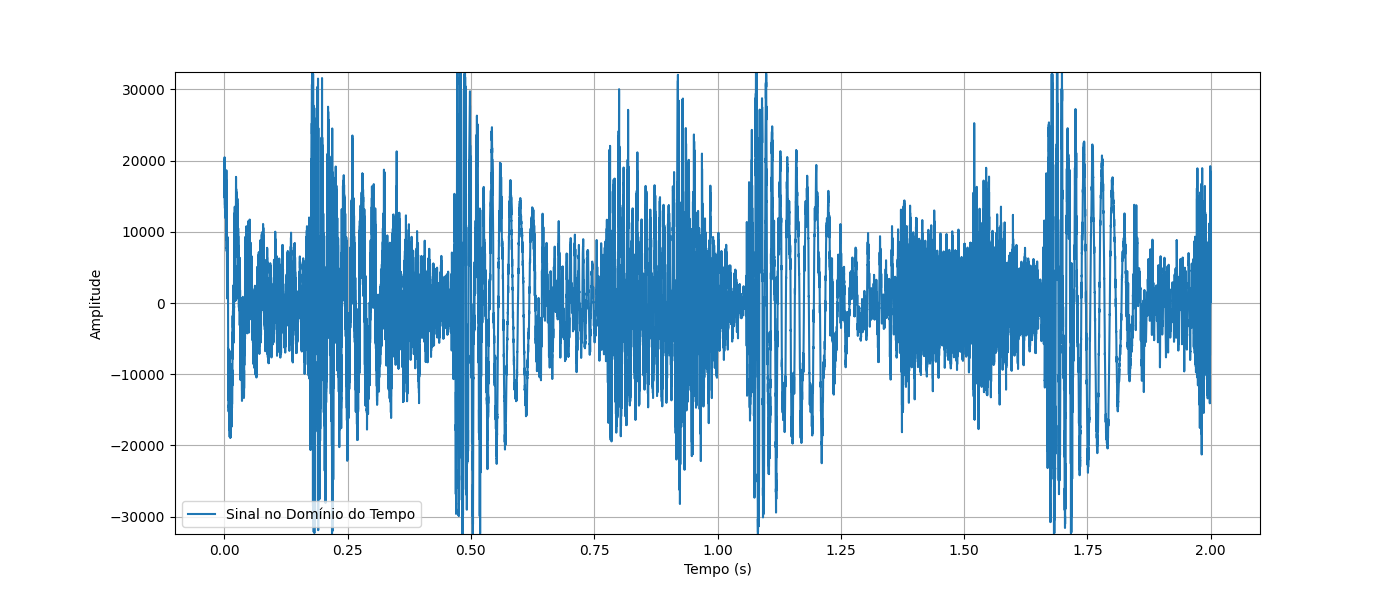
\includegraphics[width=\textwidth]{figuras/fig40.png}
        \vspace{0.3cm} % Espaço entre imagem e sublegenda
        (a) Domínio do tempo.
    \end{minipage}
    \hspace{0.5cm} % Espaço horizontal entre as figuras

    % Subfigura b
    \begin{minipage}[b]{0.7\textwidth}
        \centering
        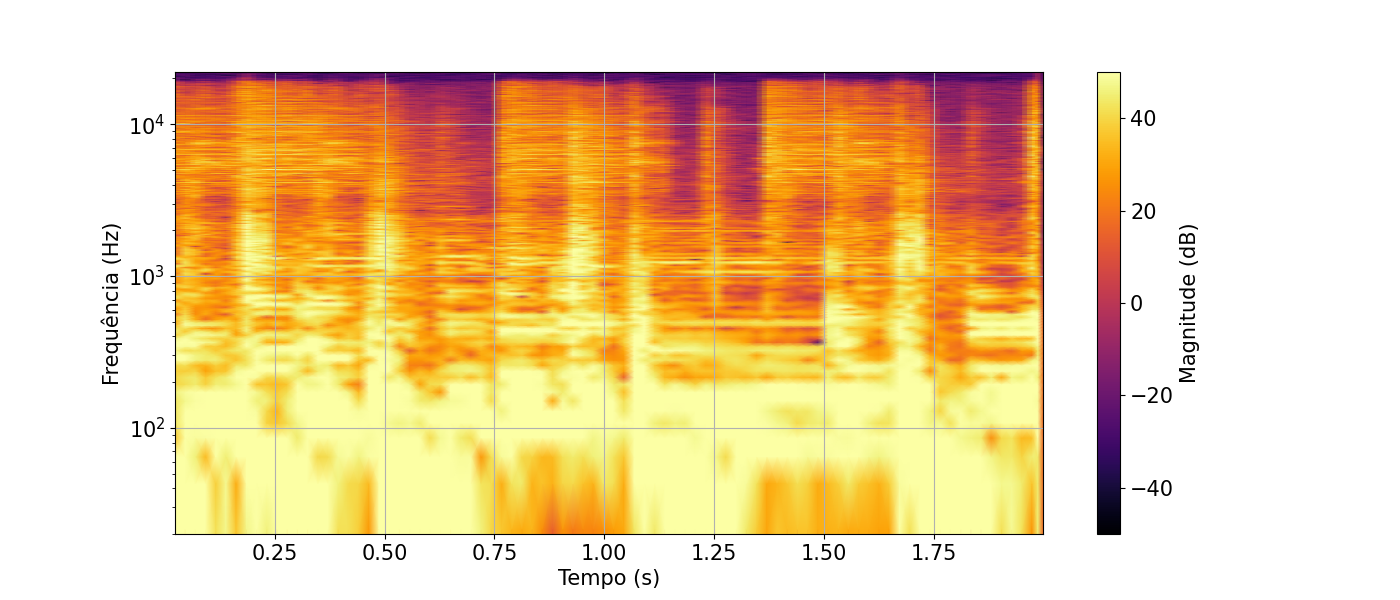
\includegraphics[width=\textwidth]{figuras/fig41.png}
        \vspace{0.3cm} % Espaço entre imagem e sublegenda
        (b) Domínio da frequência.
    \end{minipage}

    % Legenda geral
    \caption{Gráfico de intervalo da Música 1 no domínio do tempo (a) e no domínio da frequência (b), ambos sem filtragem.}
    \label{fig40}
\end{figure}







\begin{figure}[htpb]
    \centering
    % Subfigura a - Domínio do Tempo
    \begin{minipage}[b]{0.7\textwidth}
        \centering
        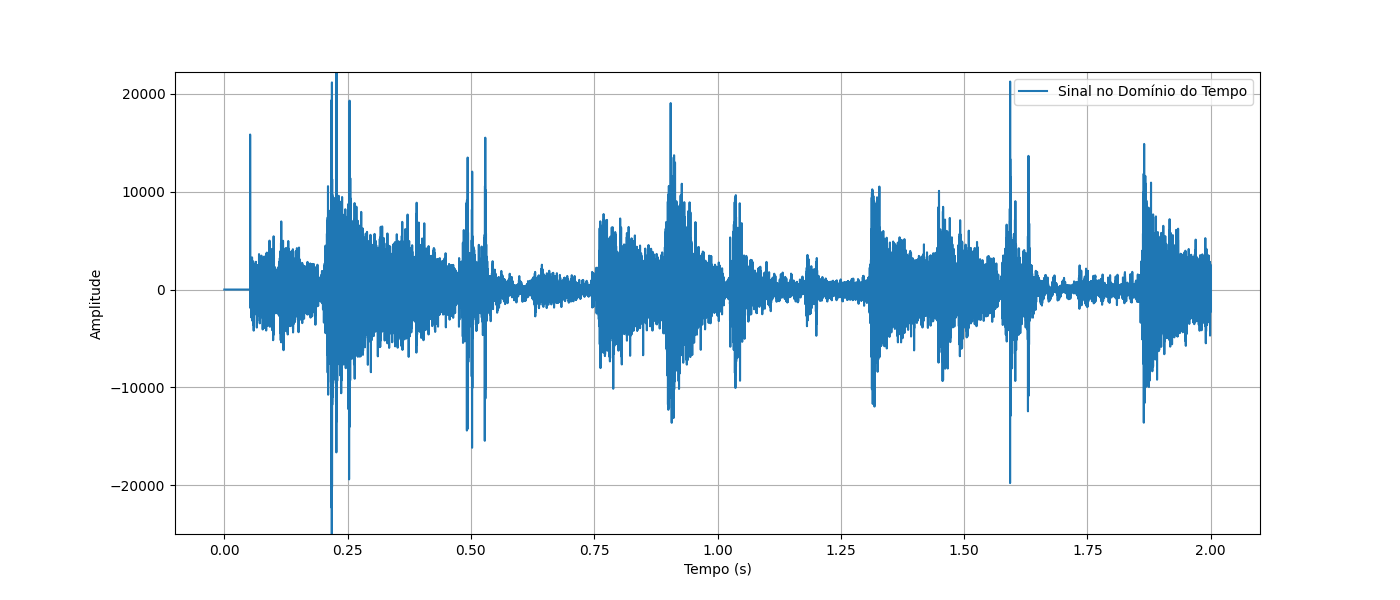
\includegraphics[width=\textwidth]{figuras/fig28.png}
        \vspace{0.3cm} % Espaço entre imagem e sublegenda
        (a) Domínio do tempo.
    \end{minipage}
    \hspace{0.5cm} % Espaço horizontal entre as figuras

    % Subfigura b - Domínio da Frequência
    \begin{minipage}[b]{0.7\textwidth}
        \centering
        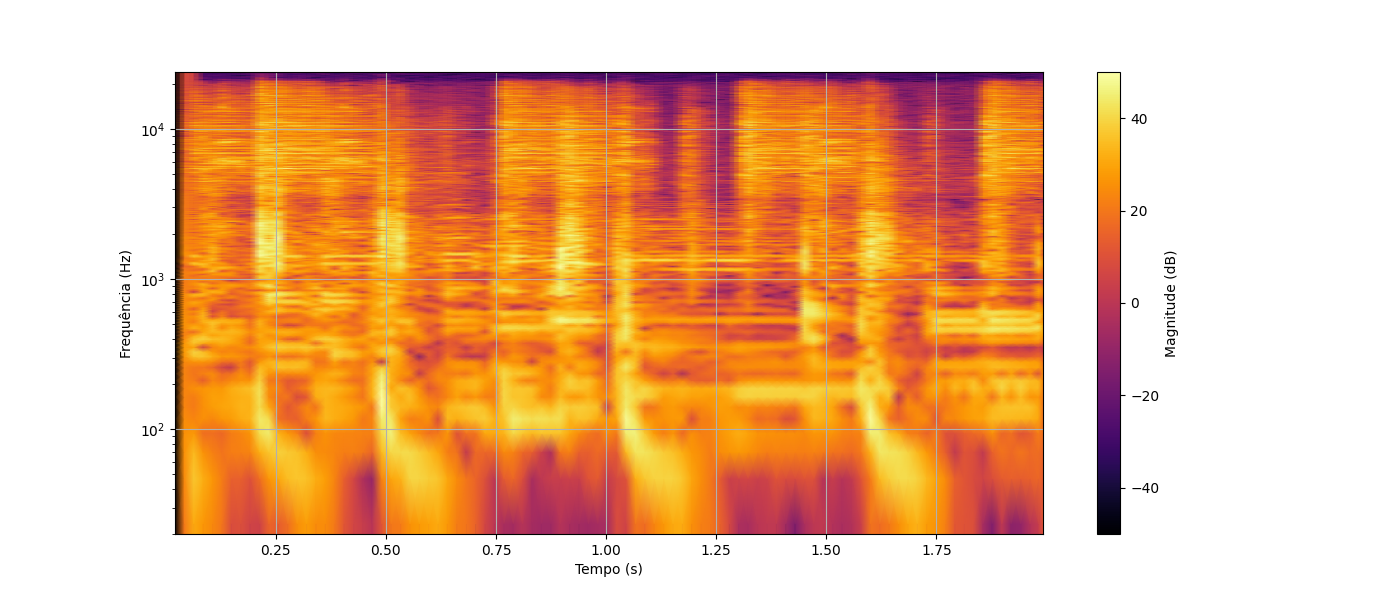
\includegraphics[width=\textwidth]{figuras/fig29.png}
        \vspace{0.3cm} % Espaço entre imagem e sublegenda
        (b) Domínio da frequência.
    \end{minipage}

    % Legenda geral
    \caption{Música 1 nos domínios do tempo (a) e da frequência (b), com uma frequência de corte de 300 Hz.}
    \label{fig28}
\end{figure}


\begin{figure}[htpb]
    \centering
    % Subfigura a - Domínio do Tempo
    \begin{minipage}[b]{0.7\textwidth}
        \centering
        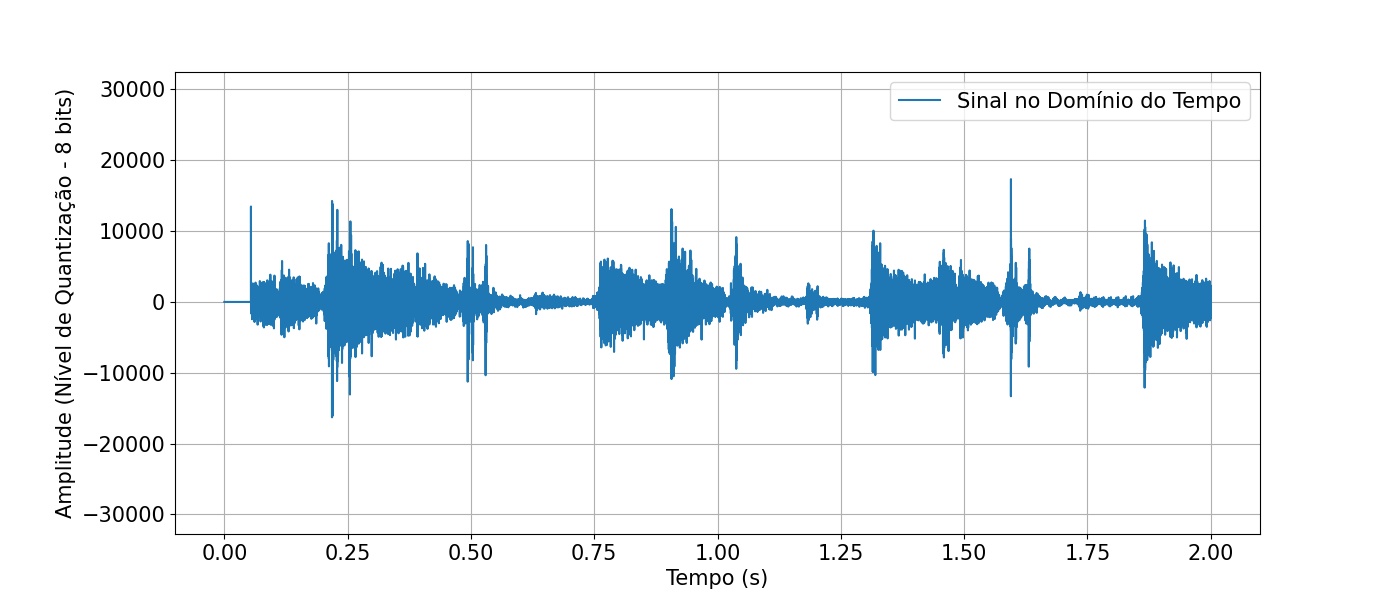
\includegraphics[width=\textwidth]{figuras/fig26.png}
        \vspace{0.3cm} % Espaço entre imagem e sublegenda
        (a) Domínio do tempo.
    \end{minipage}
    \hspace{0.5cm} % Espaço horizontal entre as figuras

    % Subfigura b - Domínio da Frequência
    \begin{minipage}[b]{0.7\textwidth}
        \centering
        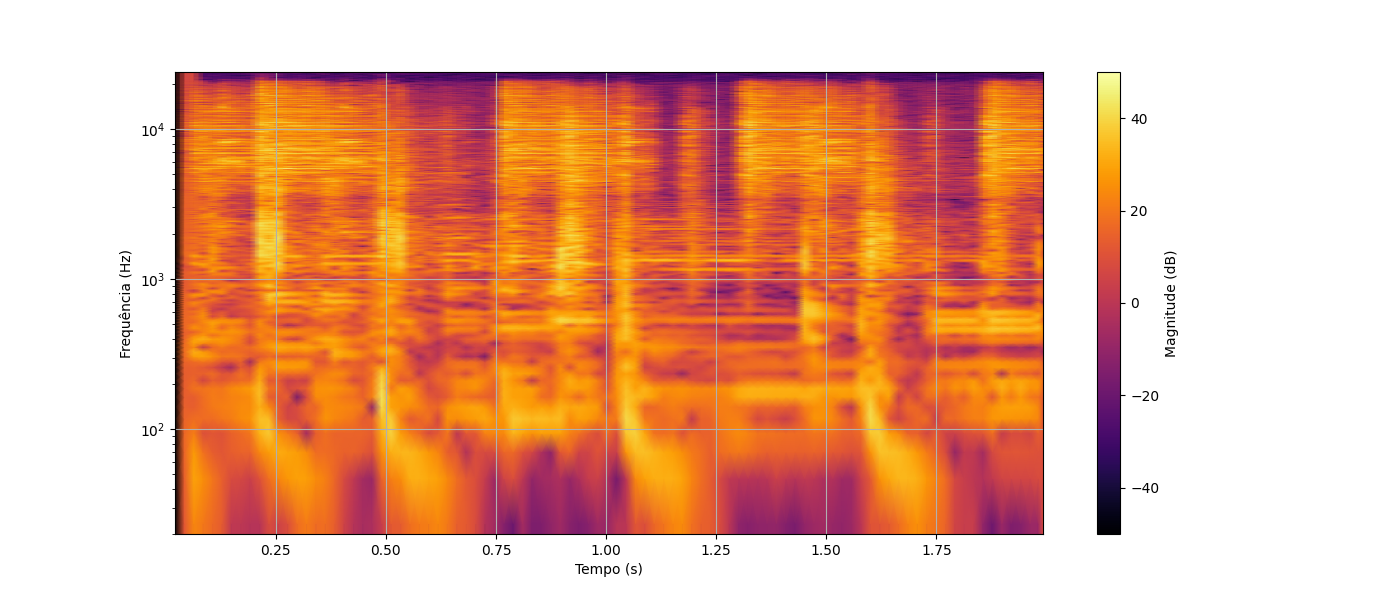
\includegraphics[width=\textwidth]{figuras/fig27.png}
        \vspace{0.3cm} % Espaço entre imagem e sublegenda
        (b) Domínio da frequência.
    \end{minipage}

    % Legenda geral
    \caption{Música 1 nos domínios do tempo (a) e da frequência (b), com uma frequência de corte de 4 kHz.}
    \label{fig26}
\end{figure}

\begin{figure}[htpb]
    \centering
    % Subfigura a - Domínio do Tempo
    \begin{minipage}[b]{0.7\textwidth}
        \centering
        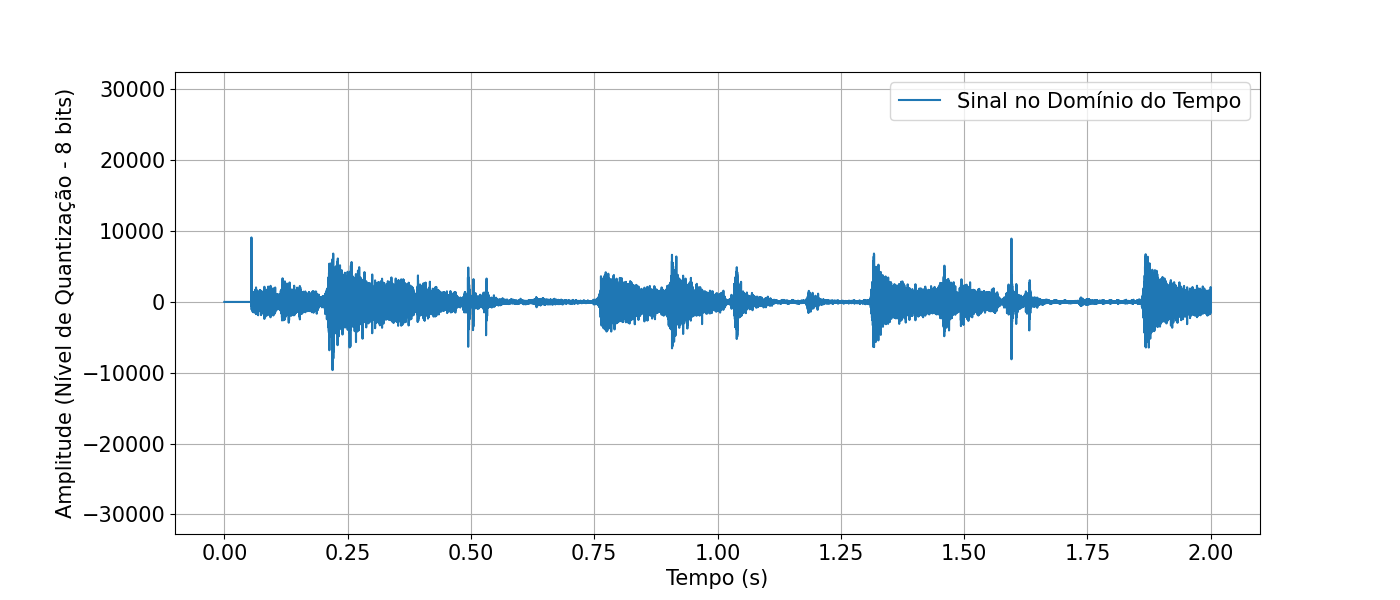
\includegraphics[width=\textwidth]{figuras/fig30.png}
        \vspace{0.3cm} % Espaço entre imagem e sublegenda
        (a) Domínio do tempo.
    \end{minipage}
    \hspace{0.5cm} % Espaço horizontal entre as figuras

    % Subfigura b - Domínio da Frequência
    \begin{minipage}[b]{0.7\textwidth}
        \centering
        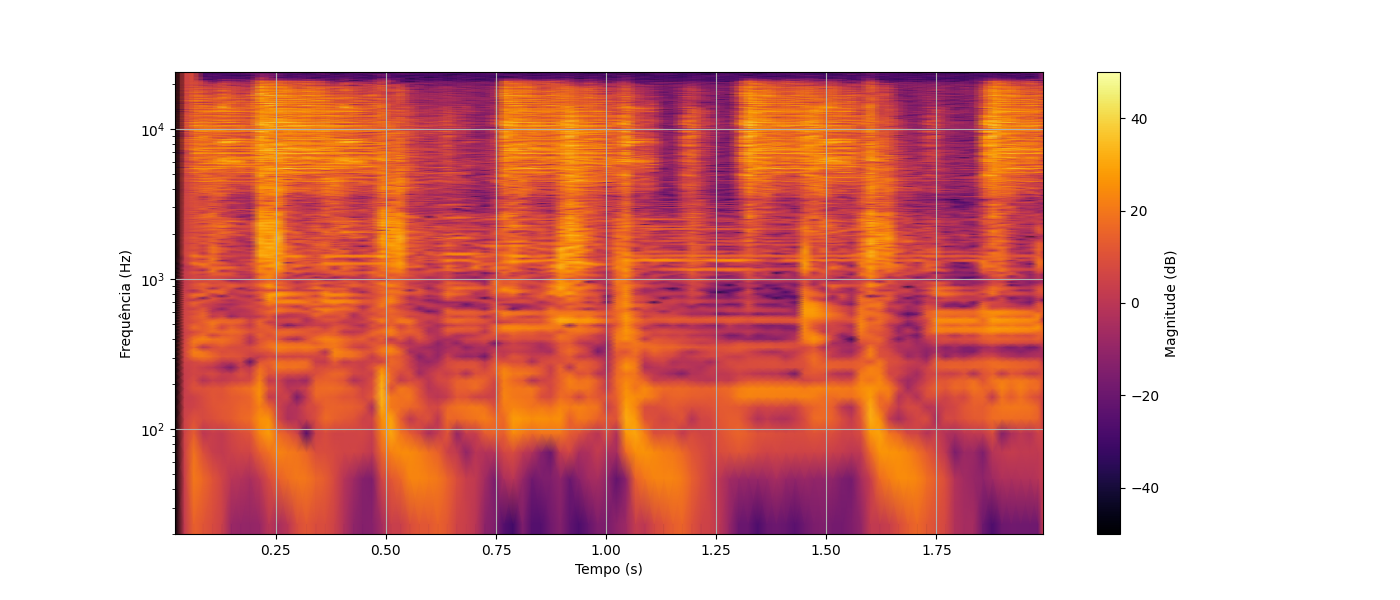
\includegraphics[width=\textwidth]{figuras/fig31.png}
        \vspace{0.3cm} % Espaço entre imagem e sublegenda
        (b) Domínio da frequência.
    \end{minipage}

    % Legenda geral
    \caption{Música 1 nos domínios do tempo (a) e da frequência (b), com uma frequência de corte de 22 kHz.}
    \label{fig30}
\end{figure}


% Na Figura \ref{fig41}, a STFT da mesma janela revela uma maior presença de elementos em baixa frequência. Assim como na Figura \ref{fig40}, é possível observar a variação de elementos agudos ao longo da música.

% \begin{figure}[h]
%     \centering
%     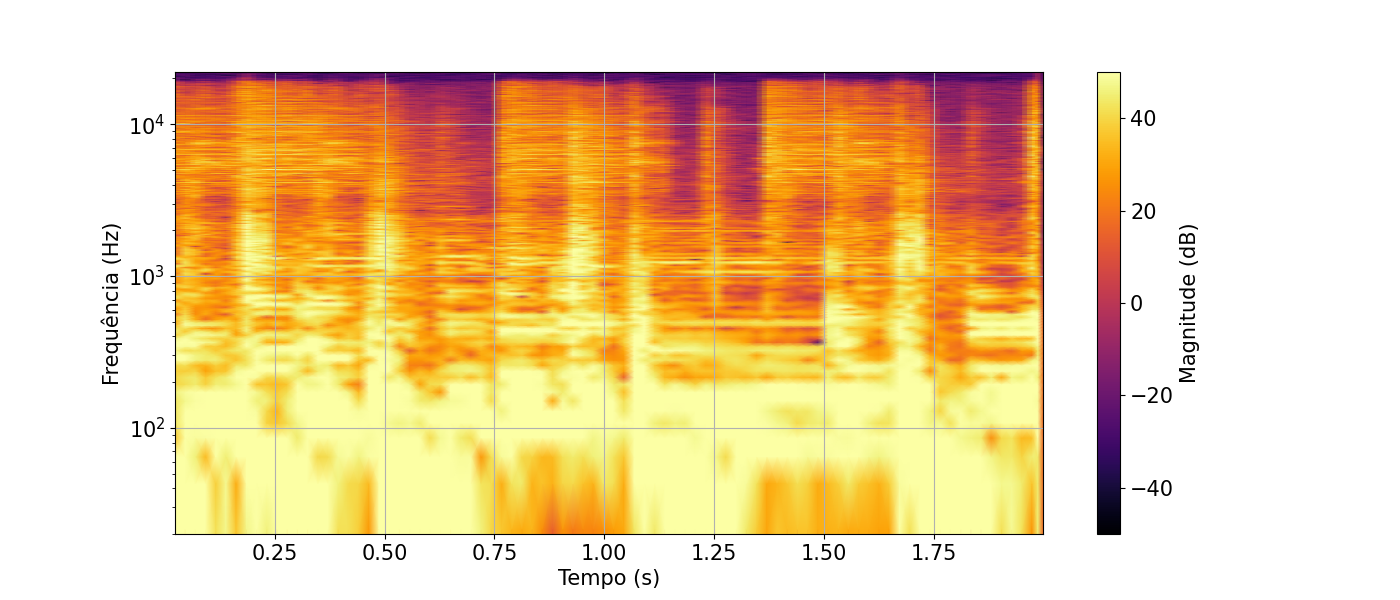
\includegraphics[width=0.7\textwidth]{figuras/fig41.png}
%     \caption{Música 1 no domínio da frequência sem filtragem}
%     \label{fig41}
% \end{figure}

% Após a aplicação de um filtro passa-altas com frequência de corte de 20 Hz, as alterações no sinal são sutis. A Figura \ref{fig24} mostra o sinal com a filtragem aplicada.

% \begin{figure}[h]
%     \centering
%     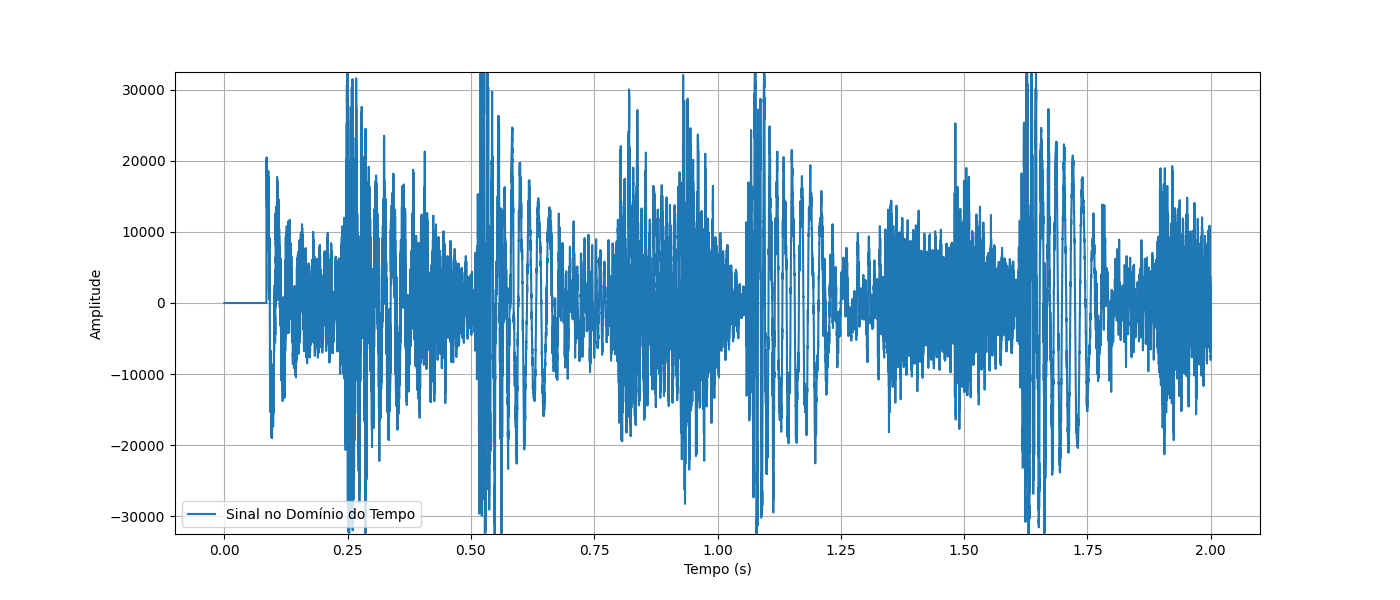
\includegraphics[width=0.7\textwidth]{figuras/fig24.png}
%     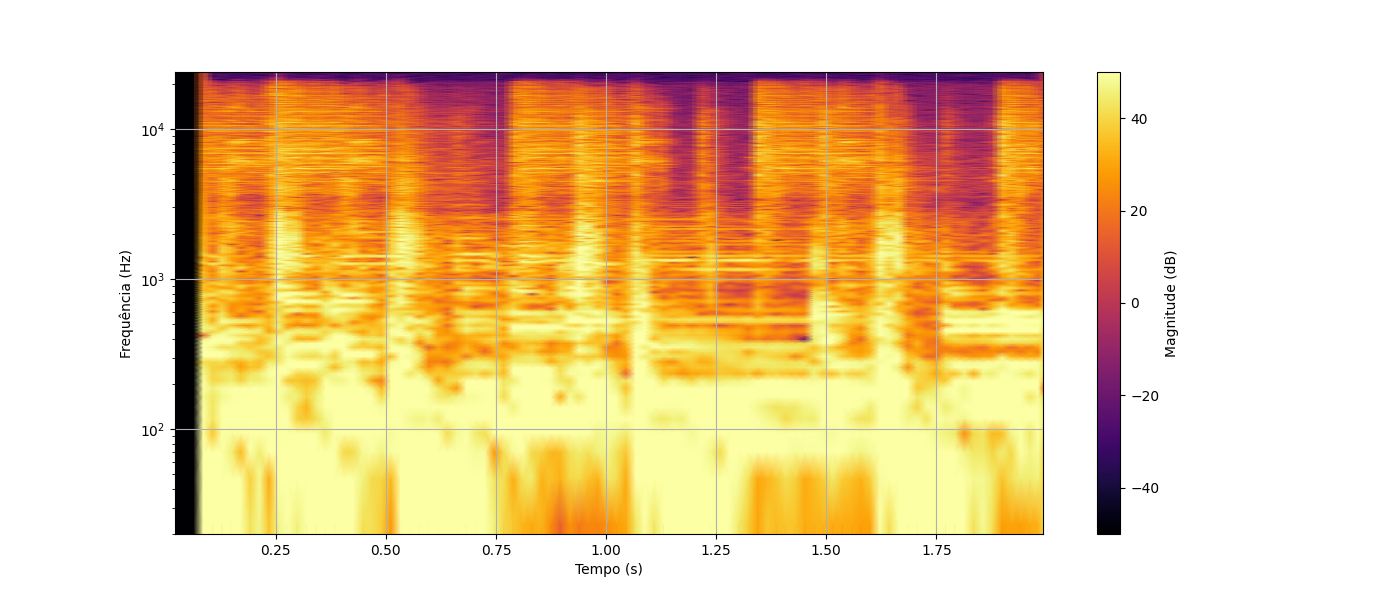
\includegraphics[width=0.75\textwidth]{figuras/fig25.png}
%     \caption{Gráfico de intervalo da Música 1 no domínio do tempo e no domínio da frequência, com frequência de corte de 20 Hz.}
%     \label{fig24}
% \end{figure}

% % A análise da Figura \ref{fig25} confirma que as componentes em frequência não sofreram grandes alterações após a aplicação do filtro passa-altas com frequência de corte de 20 Hz.

% % \begin{figure}[h]
% %     \centering
% %     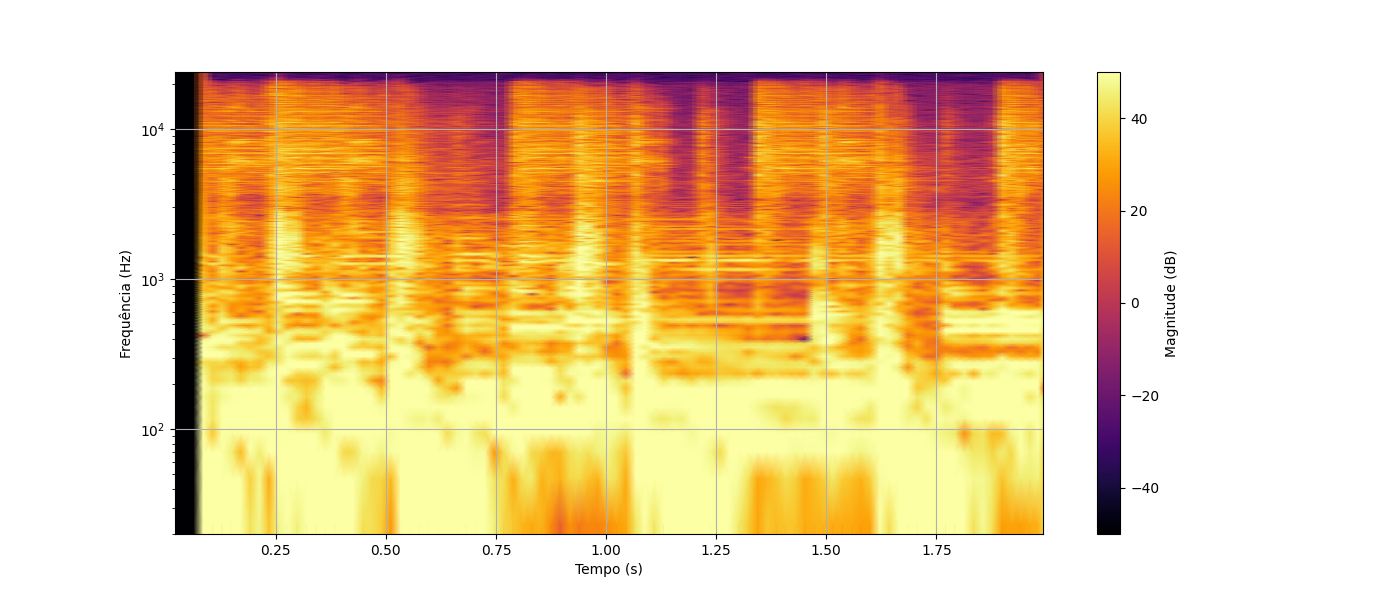
\includegraphics[width=0.7\textwidth]{figuras/fig25.png}
% %     \caption{Música 1 no domínio da frequência com frequência de corte de 20 Hz}
% %     \label{fig25}
% % \end{figure}


% Em \textit{mixers} convencionais, o botão correspondente às baixas frequências geralmente controla a banda de 300 Hz. Portanto, no presente estudo, o controle de frequência foi ajustado para aproximar a frequência de corte de 300 Hz.

Os resultados das filtragens em 300, 4000 e 22000 Hz podem ser visualizados nas Figs. \ref{fig28} a \ref{fig30}, mostrando % e \ref{fig29}. A Figura \ref{fig28} mostra
que houve uma atenuação significativa dos sinais, evidenciada pelos valores máximos da amplitude. Observa-se também a ausência de sinais de baixa frequência, que estavam presentes como envelopes nos sinais não-filtrados.

% A atenuação da banda de 300 Hz é confirmada na Figura \ref{fig29}, onde se observa uma redução de aproximadamente 30 dB nas componentes de baixa frequência.

% \begin{figure}[h]
%     \centering
%     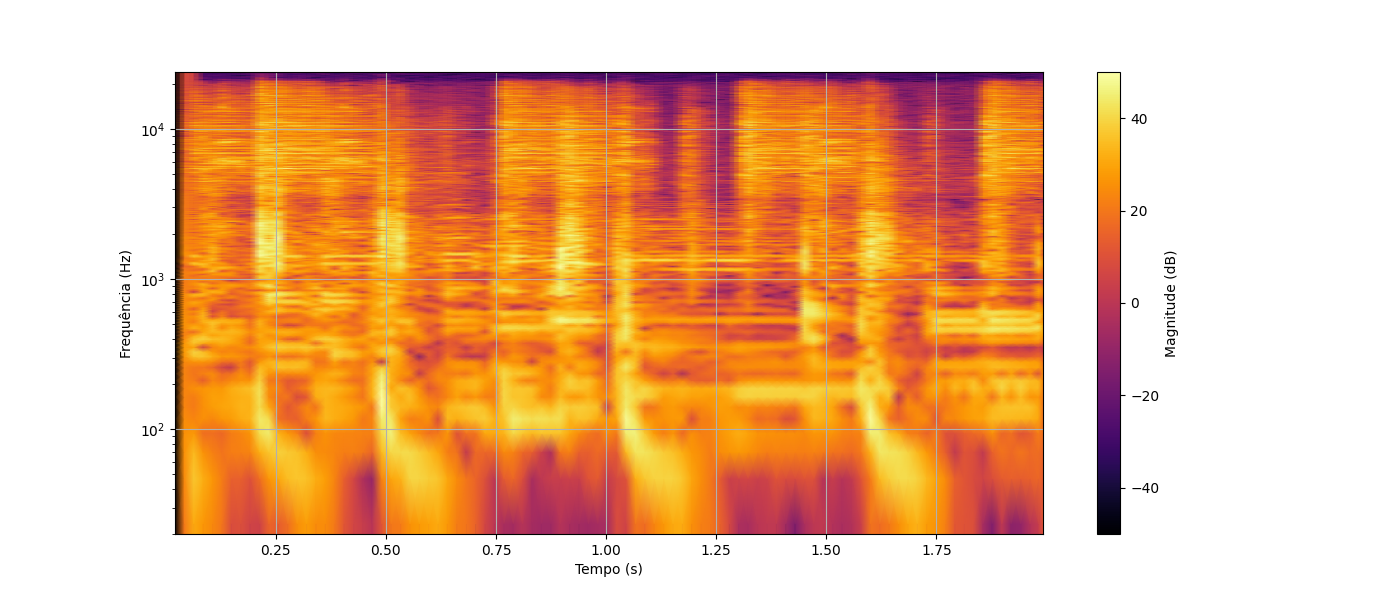
\includegraphics[width=0.7\textwidth]{figuras/fig29.png}
%     \caption{Música 1 no domínio da frequência com uma frequência de corte de 300 Hz}
%     \label{fig29}
% \end{figure}

% A próxima frequência de corte utilizada foi de 4 kHz, que, conforme descrito no Capítulo \ref{cha:fundamentacao}, é onde se encontram os elementos médios. 
% A Figura \ref{fig26} mostra a atenuação dos sinais em comparação com as filtragens anteriores.

% \begin{figure}[h]
%     \centering
%     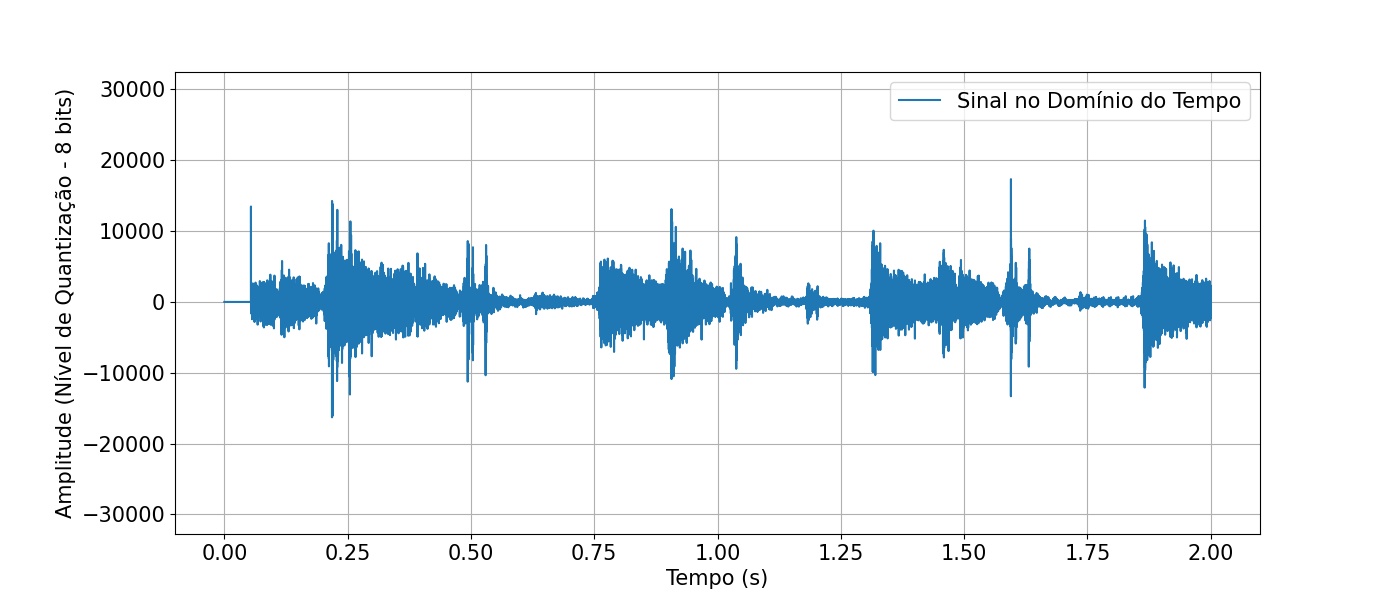
\includegraphics[width=0.7\textwidth]{figuras/fig26.png}
%     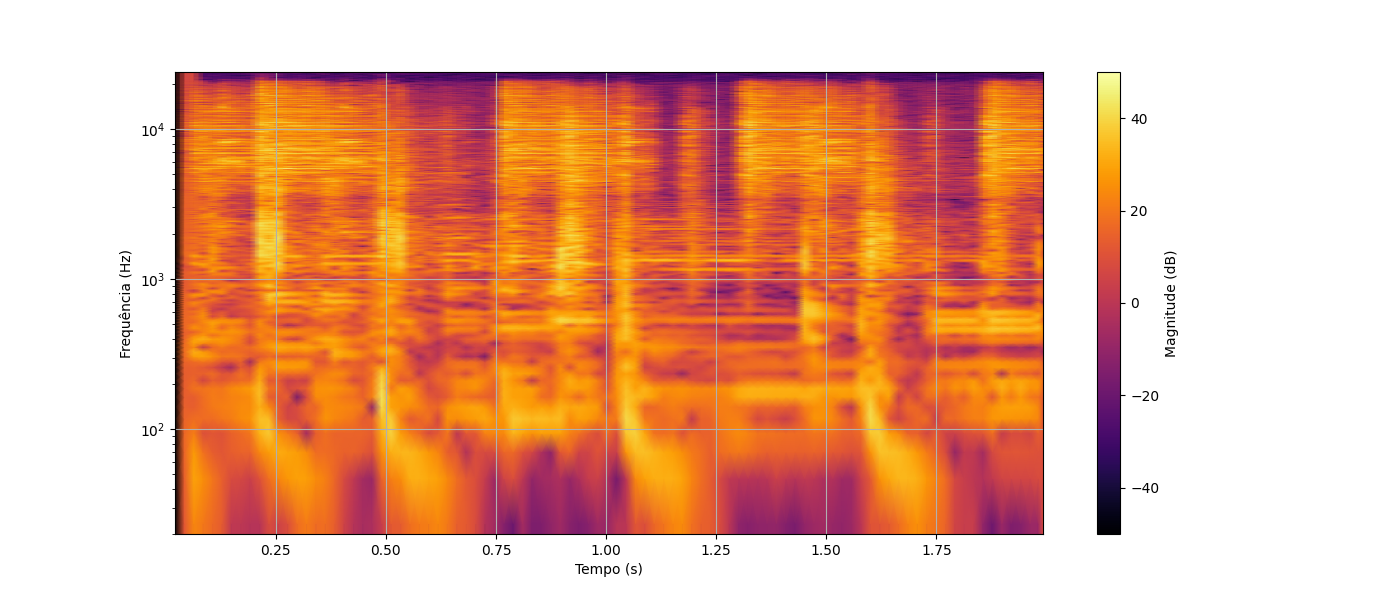
\includegraphics[width=0.75\textwidth]{figuras/fig27.png}
%     \caption{Música 1 nos domínios do tempo e da frequência, com uma frequência de corte de 4 kHz.}
%     \label{fig26}
% \end{figure}

% Na Figura \ref{fig27}, que apresenta a STFT, observa-se uma atenuação significativa das componentes na banda de 4 kHz, com algumas componentes chegando a 0 dB em determinados pontos.

% \begin{figure}[h]
%     \centering
%     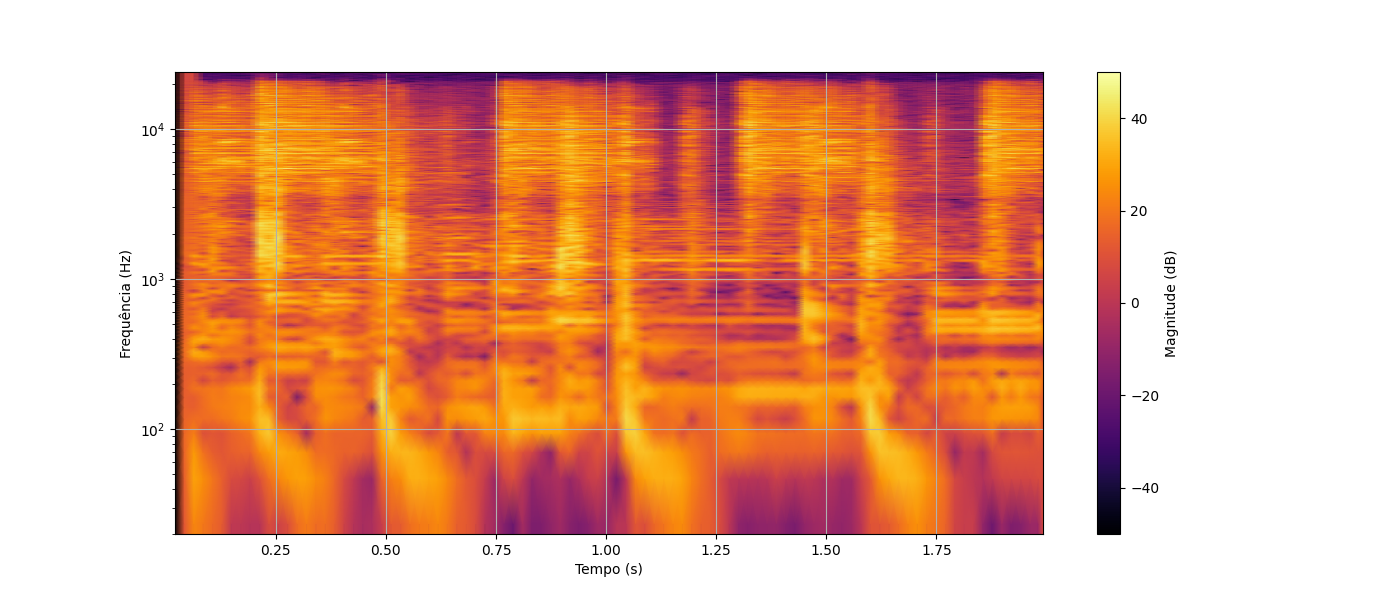
\includegraphics[width=0.7\textwidth]{figuras/fig27.png}
%     \caption{Música 1 no domínio da frequência com uma frequência de corte de 4 kHz}
%     \label{fig27}
% \end{figure}

% Para a música 1 \cite{track01}, uma análise final foi realizada utilizando uma frequência de corte de 24 kHz. Este ajuste visou atenuar os elementos restantes, considerados agudos ou brilhantes. A Figura \ref{fig30} mostra a atenuação das amplitudes dos sinais em comparação com as filtragens anteriores.

% \begin{figure}[h]
%     \centering
%     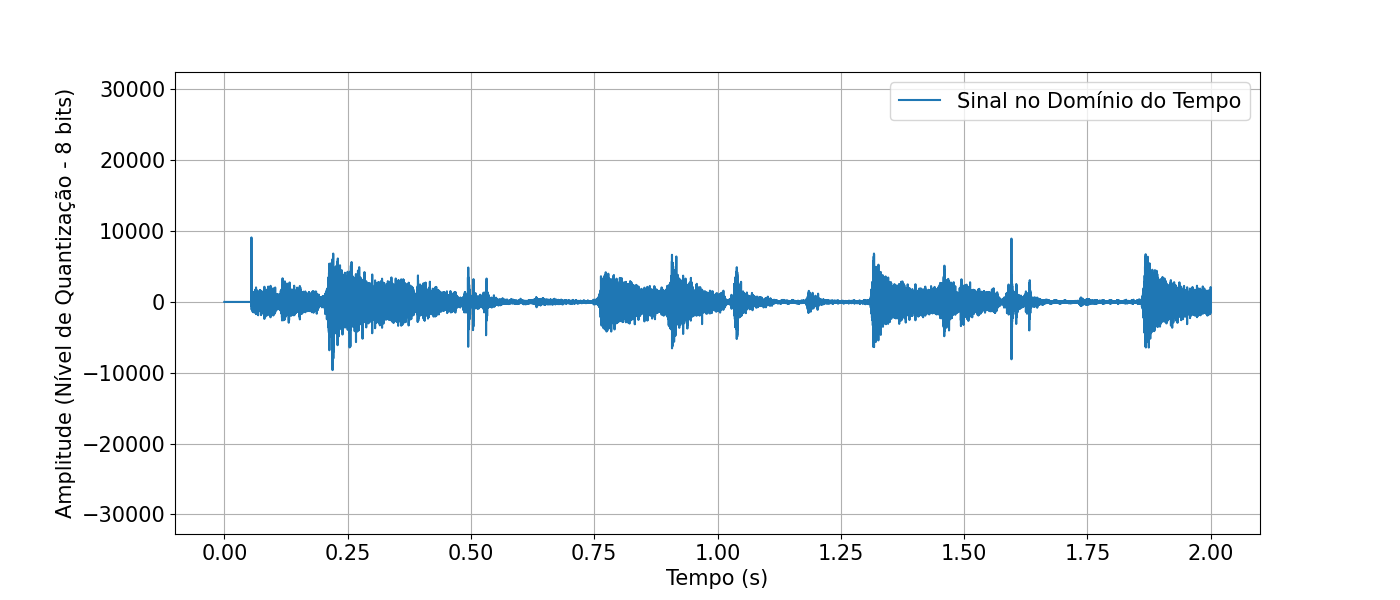
\includegraphics[width=0.7\textwidth]{figuras/fig30.png}
%     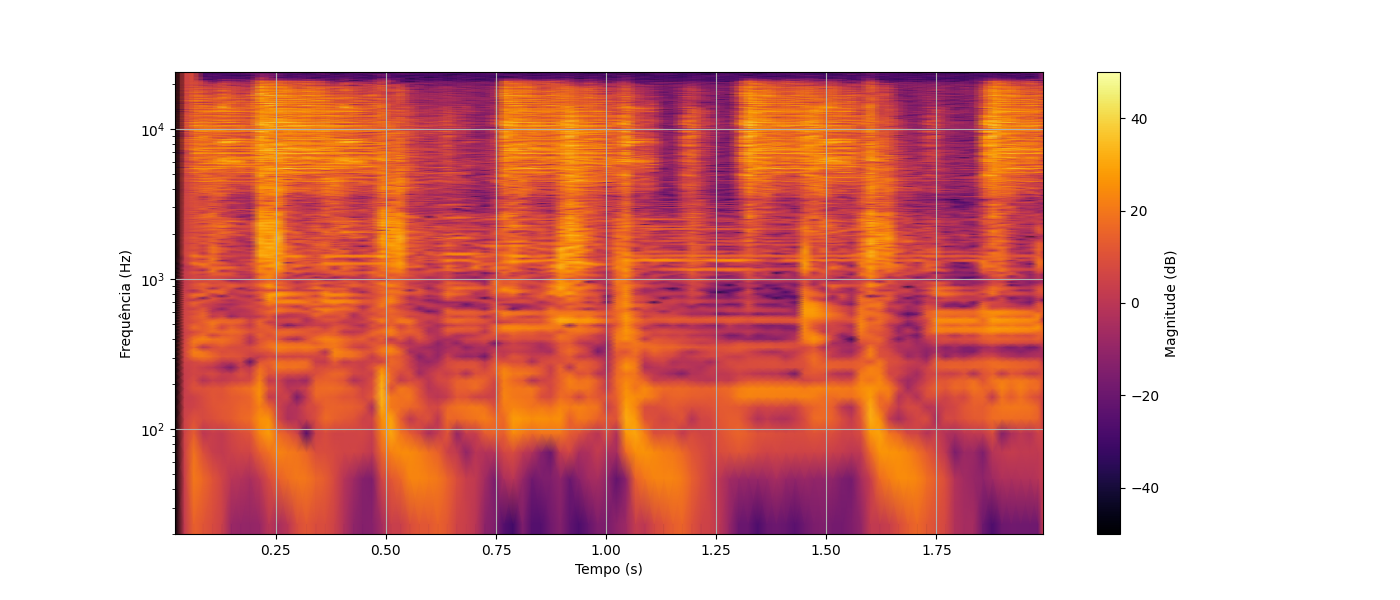
\includegraphics[width=0.75\textwidth]{figuras/fig31.png}
%     \caption{Música 1 nos domínios do tempo e da frequência, com uma frequência de corte de 22 kHz.}
%     \label{fig30}
% \end{figure}

% Além disso, na Figura \ref{fig31}, observa-se a atenuação da banda correspondente, com elementos variando de 10 dB a -40 dB. Comparado com a STFT da filtragem anterior, nota-se uma atenuação generalizada do sinal.

% \begin{figure}[h]
%     \centering
%     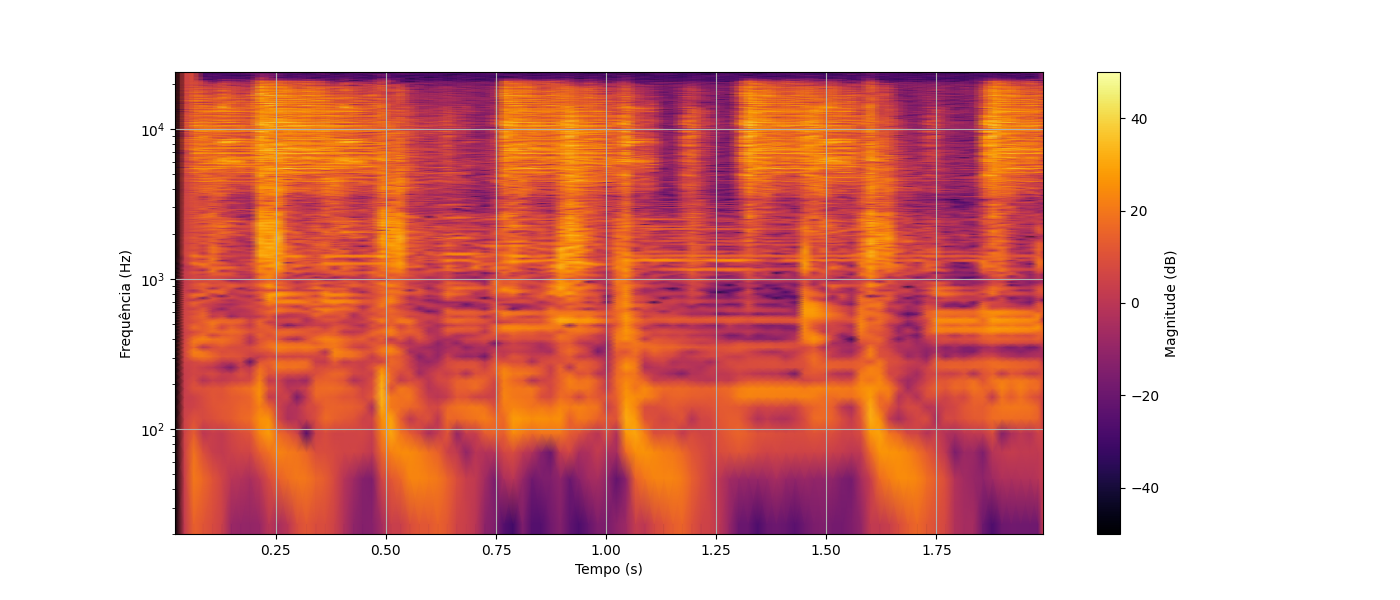
\includegraphics[width=0.7\textwidth]{figuras/fig31.png}
%     \caption{Música 1 no domínio da frequência com uma frequência de corte de 22 kHz}
%     \label{fig31}
% \end{figure}

A análise realizada na música 1 %\cite{track01}
foi também aplicada à música 2. %\cite{track02}. 
Os resultados obtidos no domínio do tempo e da frequência, utilizando a STFT, foram semelhantes aos observados para a música \cite{track01}. É importante notar que, conforme o botão de frequência de corte avança, a frequência de corte do filtro do canal 1 aumenta, atenuando primeiro as menores frequências e, em seguida, as maiores frequências. Em contraste, para o canal 2, a frequência de corte começa alta e diminui, ampliando as componentes de frequência do sinal da música \cite{track02}.

%\newpage
\subsection{Efeitos}

Os efeitos são controlados pela frequência central, que determina o volume do efeito, e um botão de duas posições, que seleciona o efeito a ser utilizado. Testes foram realizados para verificar essas operações.
Primeiramente, simulou-se o volume do efeito em função da posição do botão central. Em seguida, foram realizadas simulações variando os parâmetros dos efeitos.

\subsubsection*{Automação de Efeitos}

\begin{figure}[htpb]
    \centering
    % Subfigura a - Volume 0.0
    \begin{minipage}[b]{0.7\textwidth}
        \centering
        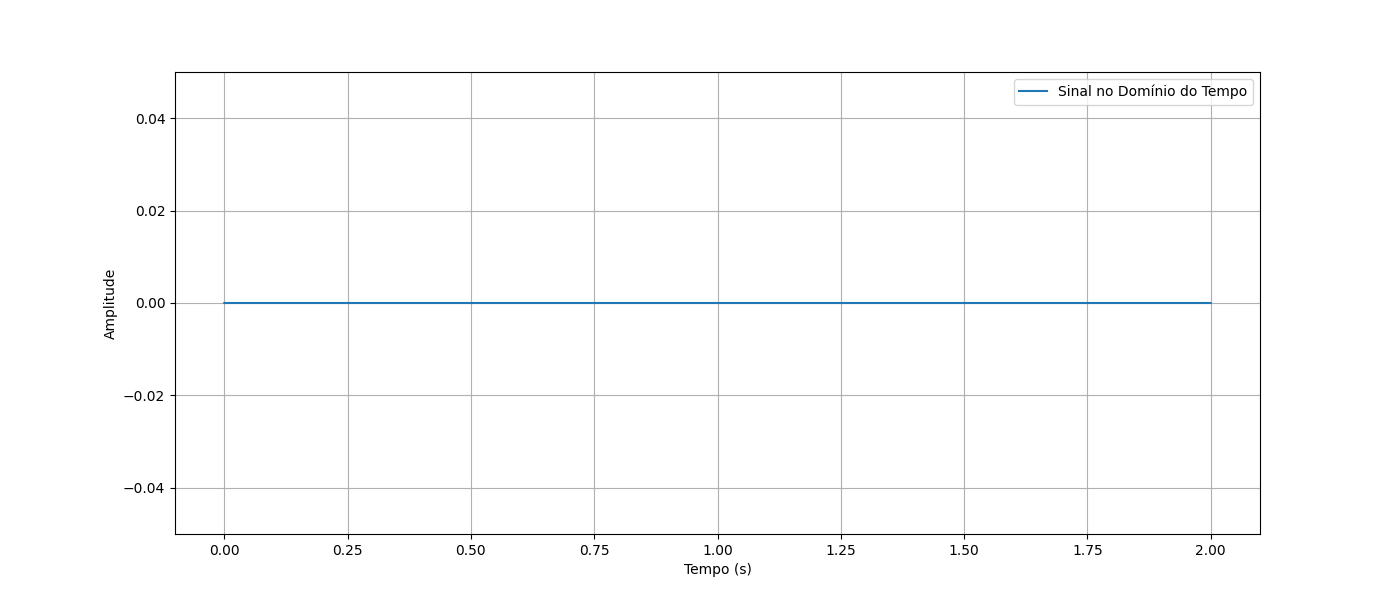
\includegraphics[width=\textwidth]{figuras/fig66.png}
        \vspace{0.3cm} % Espaço entre imagem e sublegenda
        (a) Volume 0.0.
    \end{minipage}
    \hspace{0.5cm} % Espaço horizontal entre as figuras

    % Subfigura b - Volume 0.3312
    \begin{minipage}[b]{0.7\textwidth}
        \centering
        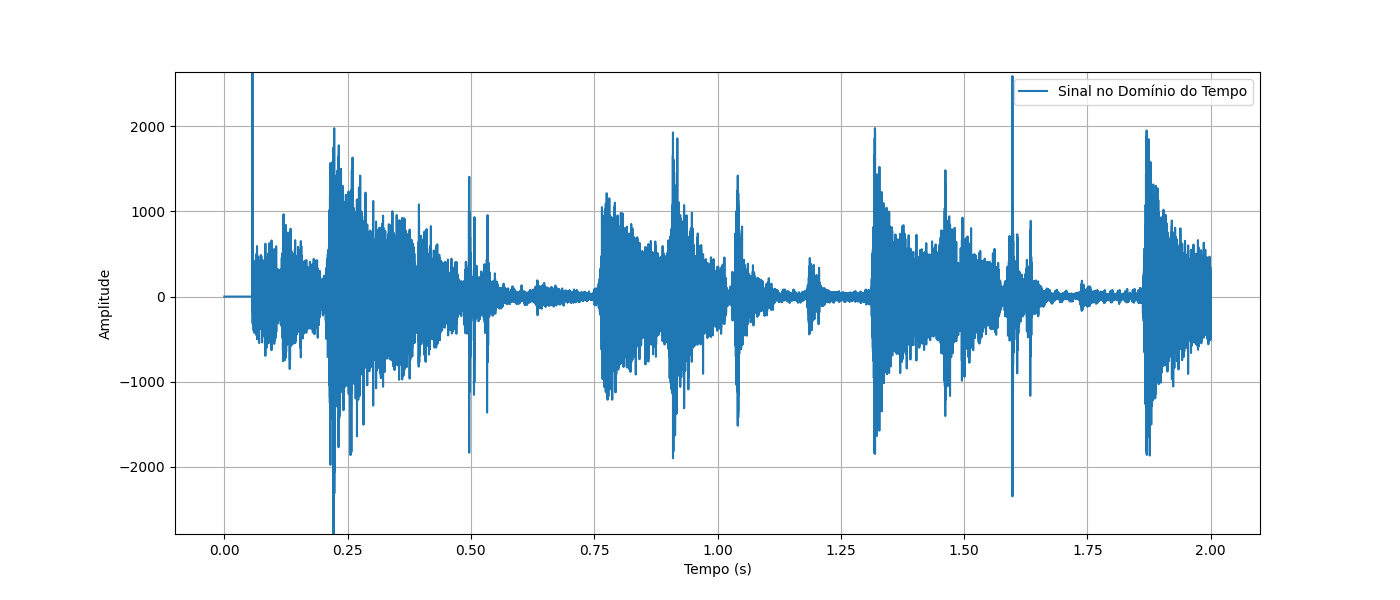
\includegraphics[width=\textwidth]{figuras/fig67.png}
        \vspace{0.3cm} % Espaço entre imagem e sublegenda
        (b) Volume 0.3312.
    \end{minipage}
    
    \vspace{0.5cm} % Espaço vertical entre as linhas de figuras

    % Subfigura c - Volume 0.6625
    \begin{minipage}[b]{0.7\textwidth}
        \centering
        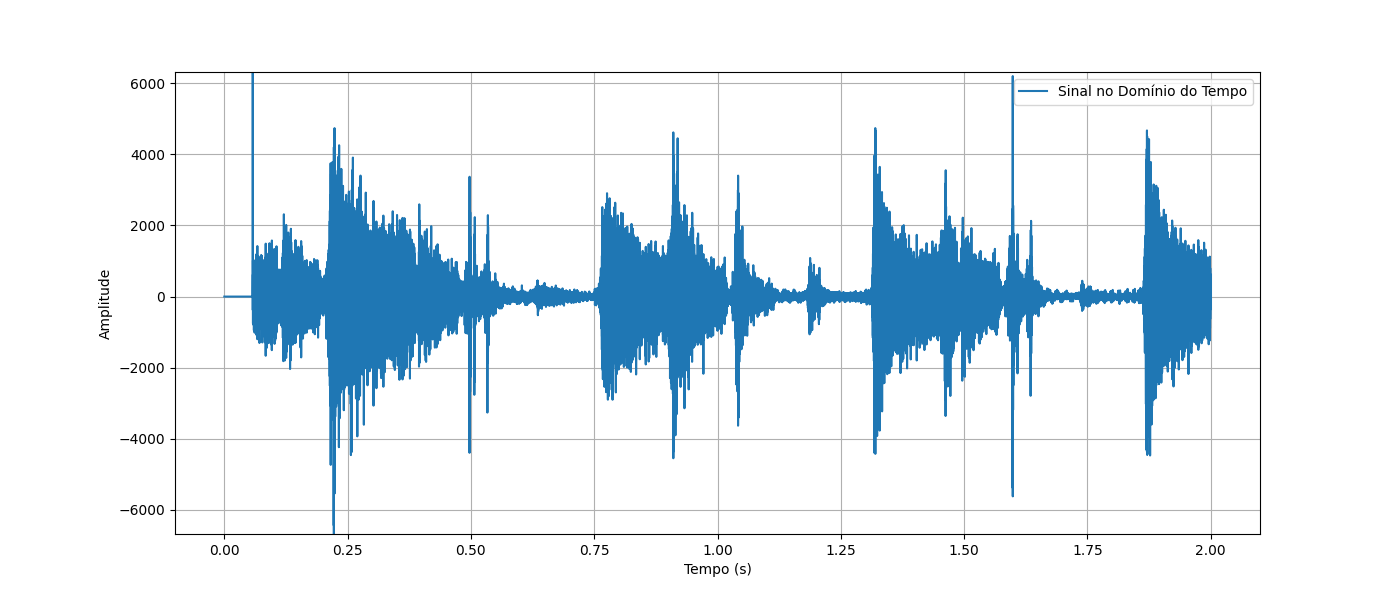
\includegraphics[width=\textwidth]{figuras/fig68.png}
        \vspace{0.3cm} % Espaço entre imagem e sublegenda
        (c) Volume 0.6625.
    \end{minipage}
    \hspace{0.5cm} % Espaço horizontal entre as figuras

    % Subfigura d - Volume 1.0
    \begin{minipage}[b]{0.7\textwidth}
        \centering
        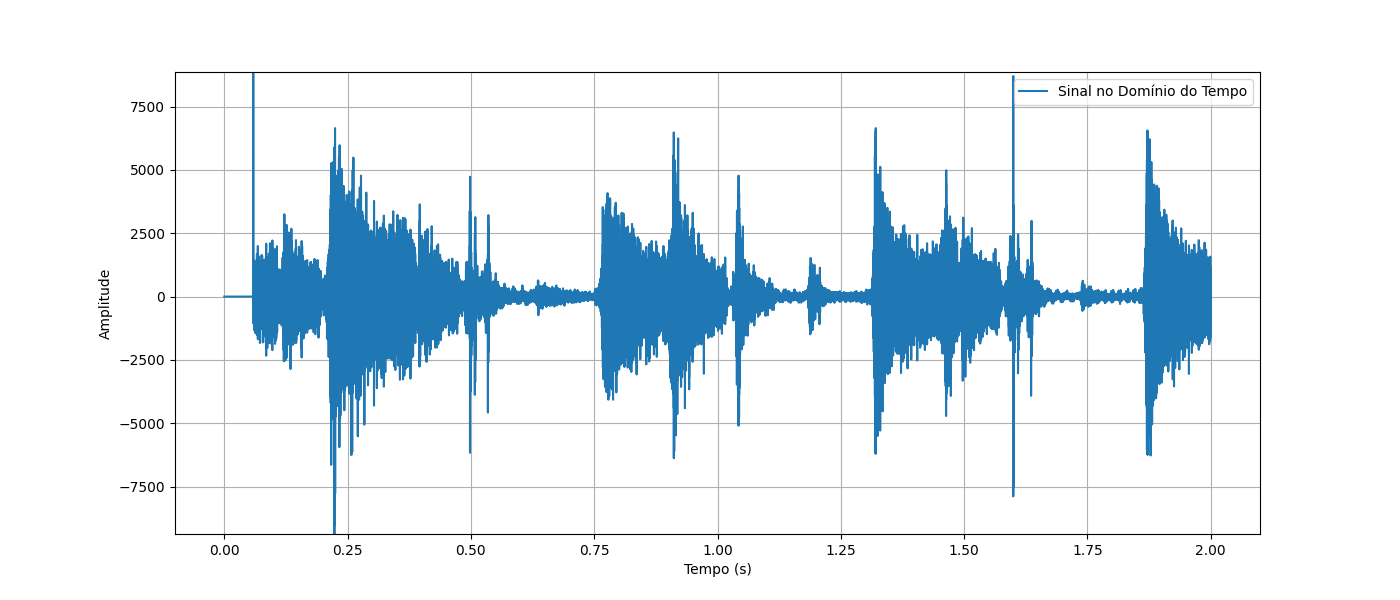
\includegraphics[width=\textwidth]{figuras/fig69.png}
        \vspace{0.3cm} % Espaço entre imagem e sublegenda
        (d) Volume 1.0.
    \end{minipage}

    % Legenda geral
    \caption{Canal de efeito \textit{reverb} isolado com música 1 a volumes de 0.0, 0.3312, 0.6625 e 1.0.}
    \label{fig66}
\end{figure}


Para validar o controle automático do volume, isolou-se a saída dos efeitos e variaram-se as frequências, que geram diferentes volumes de efeitos, %. Os sinais no domínio do tempo foram analisados, 
conforme mostrado na Fig. \ref{fig66}.
A frequência central foi aumentada gradativamente, indo de um sinal constante e nulo na frequência de corte de 0 Hz, para 0,3312 (9454 Hz), 0,6625 (9875 Hz) e 1,0 (11025 Hz). Repare como as amplitudes dos sinais da Fig. \ref{fig66} aumentam gradativamente.

% \begin{figure}[h]
%     \centering
%     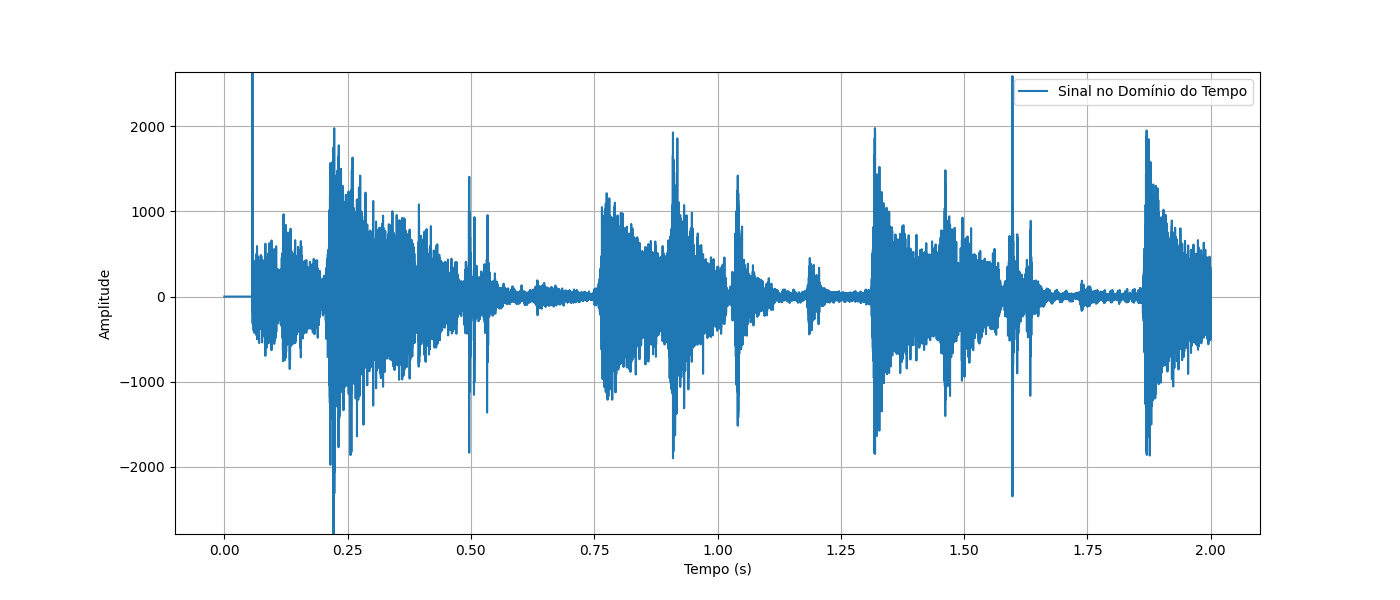
\includegraphics[width=0.7\textwidth]{figuras/fig67.png}
%     \caption{canal de efeito \textit{reverb} isolado com música 1 a um volume de 0.3312}
%     \label{fig67}
% \end{figure}

% Em seguida, variou-se a posição do botão central para atingir a frequência de 9454 Hz, resultando em um volume de 0.3312. A Figura \ref{fig67} mostra um sinal similar ao da música \cite{track01}, mas com uma amplitude específica.

%\newpage

% \begin{figure}[h]
%     \centering
%     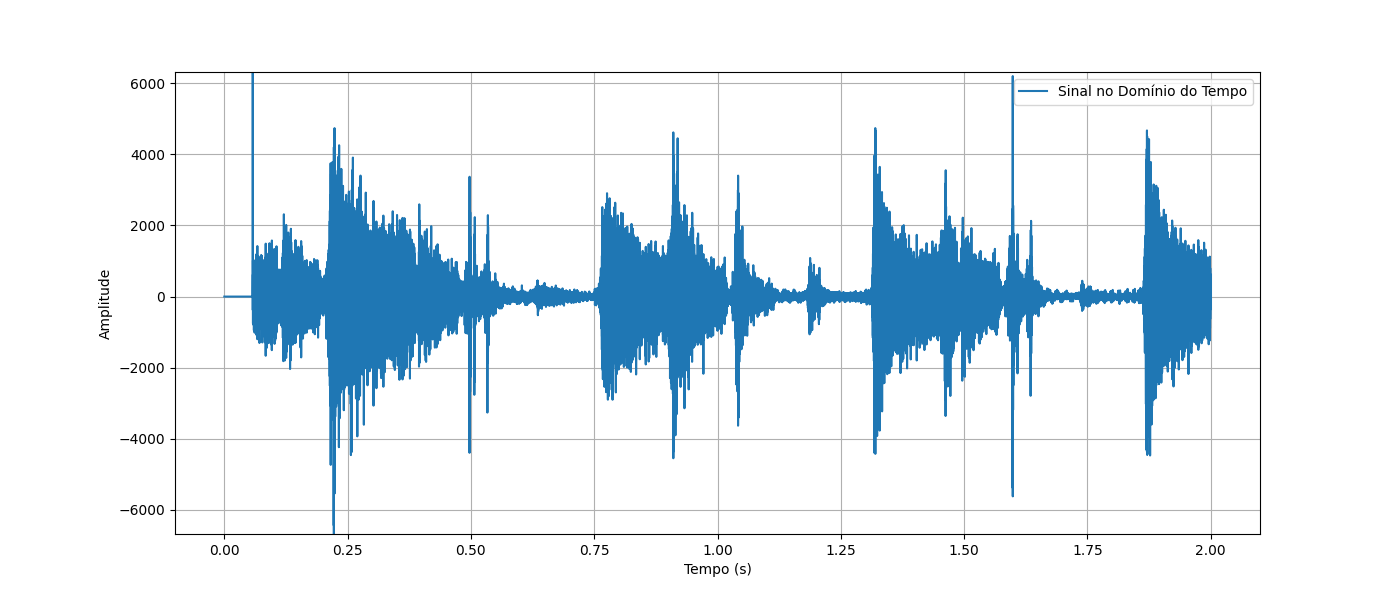
\includegraphics[width=0.7\textwidth]{figuras/fig68.png}
%     \caption{canal de efeito \textit{reverb} isolado com música 1 a um volume de 0.6625}
%     \label{fig68}
% \end{figure}

% A posição do botão central foi ajustada para observar a variação do volume do efeito. Na Figura \ref{fig68}, com a frequência de 9875 Hz, observou-se um volume maior.

% \begin{figure}[h]
%     \centering
%     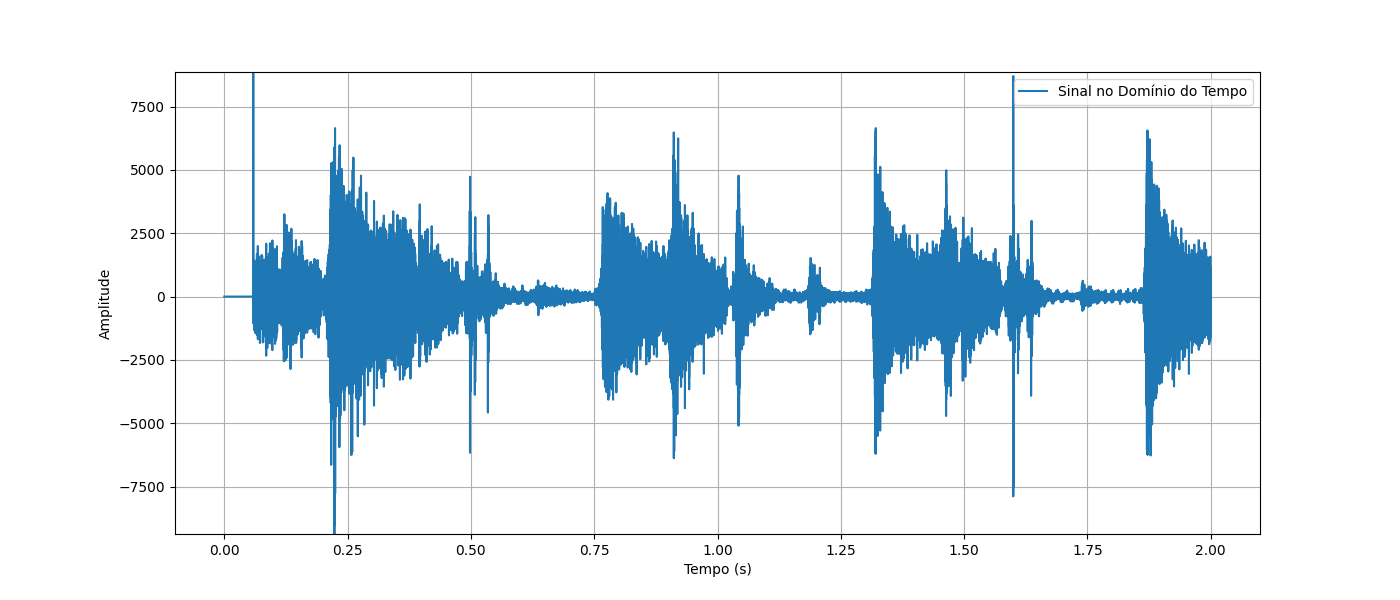
\includegraphics[width=0.7\textwidth]{figuras/fig69.png}
%     \caption{canal de efeito \textit{reverb} isolado com música 1 a um volume de 1.0}
%     \label{fig69}
% \end{figure}
% Para validar completamente a automação do volume, o botão central foi posicionado na frequência de 11025 Hz, que gera o volume máximo (1.0). A Figura \ref{fig69} mostra a ampliação do volume em função da variação da frequência, confirmando a automação do volume.

\subsubsection*{\textit{Reverb}}

Para validar o controle do efeito de \textit{reverb}, o botão central foi posicionado para garantir que a frequência selecionada resultasse no volume máximo do efeito. Em seguida, ajustou-se a posição do botão de presença do efeito para observar a variação dos parâmetros. No caso do \textit{reverb}, a quantidade de dB presente após 1 segundo é configurada conforme o botão de parâmetro.

Nas Fig. \ref{fig70}, são apresentadas representações do sinal no domínio do tempo, ilustrando a variação desse parâmetro. O intervalo de dB proposto no sistema varia de 0 a 100 dB. O efeito de \textit{reverb} foi cada vez mais pronunciado, resultando em um som com pouca definição no último gráfico, comprometendo a clareza da música.


\begin{figure}[htpb]
    \centering
    % Subfigura a - 0 dB
    \begin{minipage}[b]{0.7\textwidth}
        \centering
        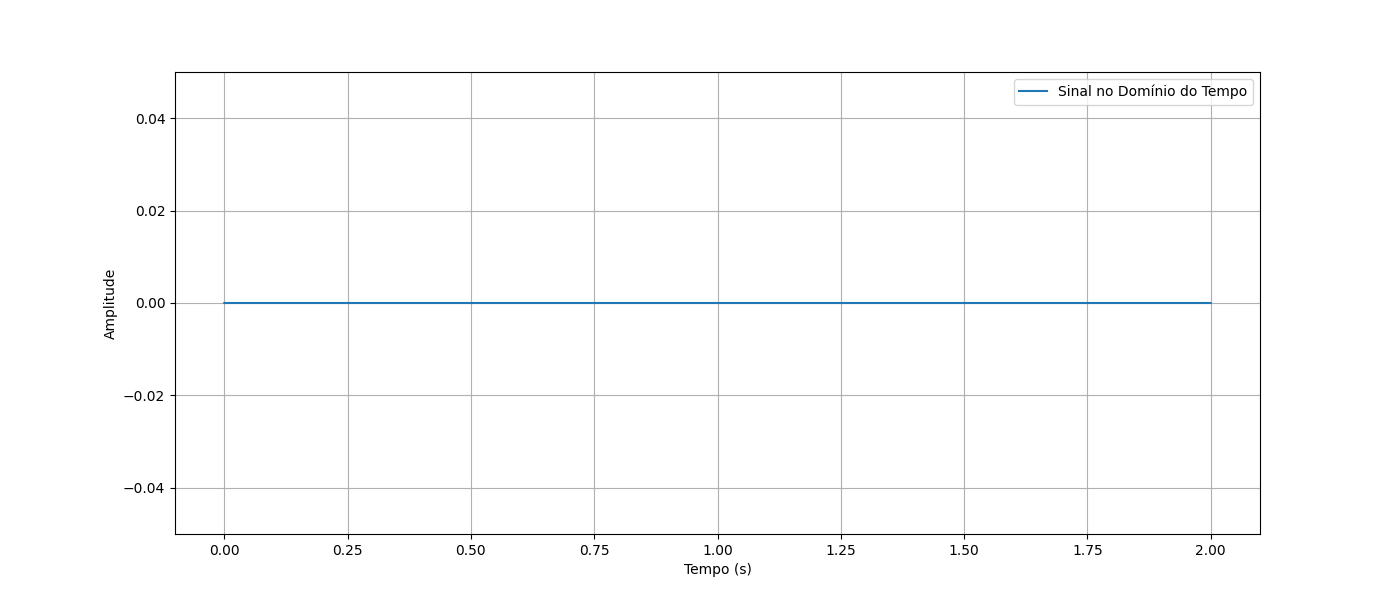
\includegraphics[width=\textwidth]{figuras/fig70.png}
        \vspace{0.3cm} % Espaço entre imagem e sublegenda
        (a) 0 dB após 1 segundo.
    \end{minipage}
    \hspace{0.5cm} % Espaço horizontal entre as figuras

    % Subfigura b - 25 dB
    \begin{minipage}[b]{0.7\textwidth}
        \centering
        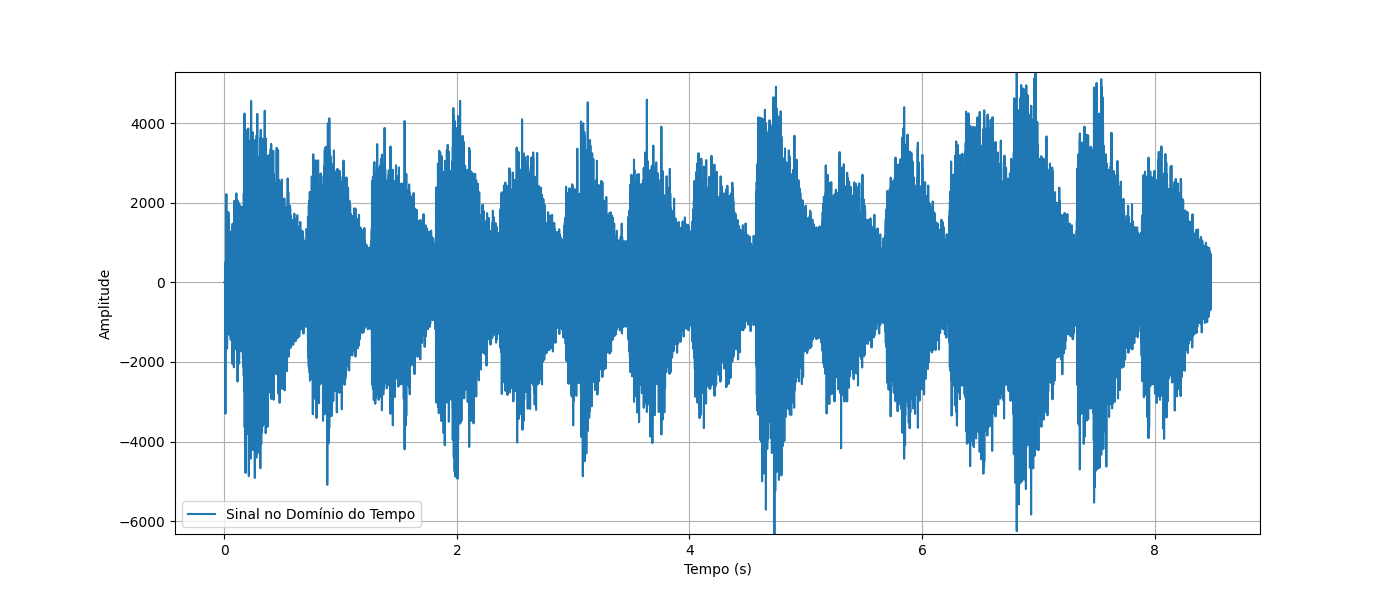
\includegraphics[width=\textwidth]{figuras/fig71.png}
        \vspace{0.3cm} % Espaço entre imagem e sublegenda
        (b) 25 dB após 1 segundo.
    \end{minipage}
    
    \vspace{0.5cm} % Espaço vertical entre as linhas de figuras

    % Subfigura c - 50 dB
    \begin{minipage}[b]{0.7\textwidth}
        \centering
        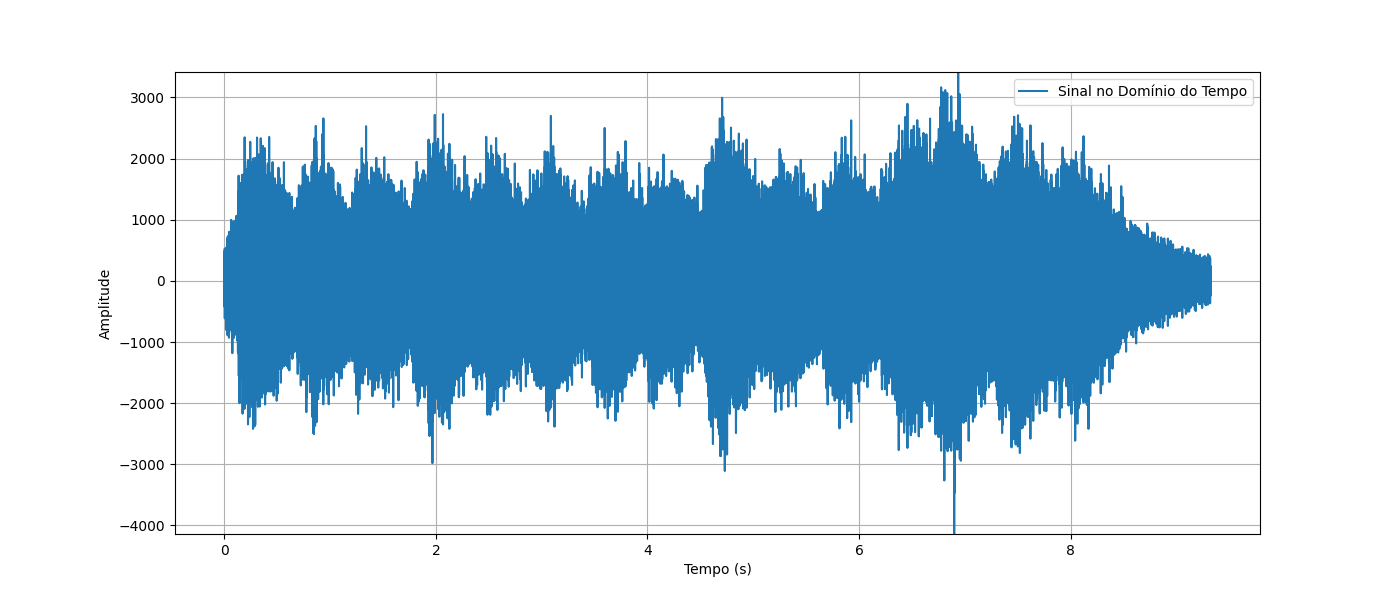
\includegraphics[width=\textwidth]{figuras/fig72.png}
        \vspace{0.3cm} % Espaço entre imagem e sublegenda
        (c) 50 dB após 1 segundo.
    \end{minipage}
    \hspace{0.5cm} % Espaço horizontal entre as figuras

    % Subfigura d - 100 dB
    \begin{minipage}[b]{0.7\textwidth}
        \centering
        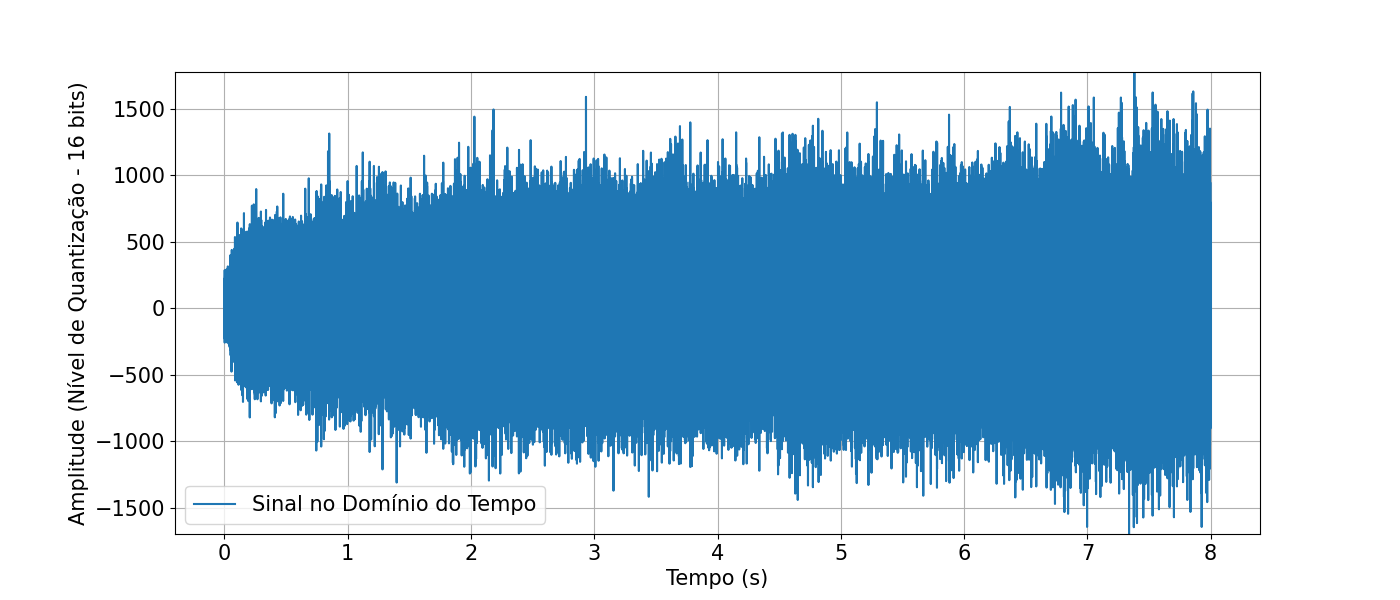
\includegraphics[width=\textwidth]{figuras/fig73.png}
        \vspace{0.3cm} % Espaço entre imagem e sublegenda
        (d) 100 dB após 1 segundo.
    \end{minipage}

    % Legenda geral
    \caption{Sinal com efeitos de \textit{reverb} a 0, 25, 50 e 100 dB após 1 segundo.}
    \label{fig70}
\end{figure}


% Na Figura \ref{fig70}, a posição inicial do botão de quantidade de efeito resulta em 0 dB após 1 segundo. Portanto, a forma de onda esperada também é nula, o que foi confirmado pelos resultados obtidos.

% \begin{figure}[h]
%     \centering
%     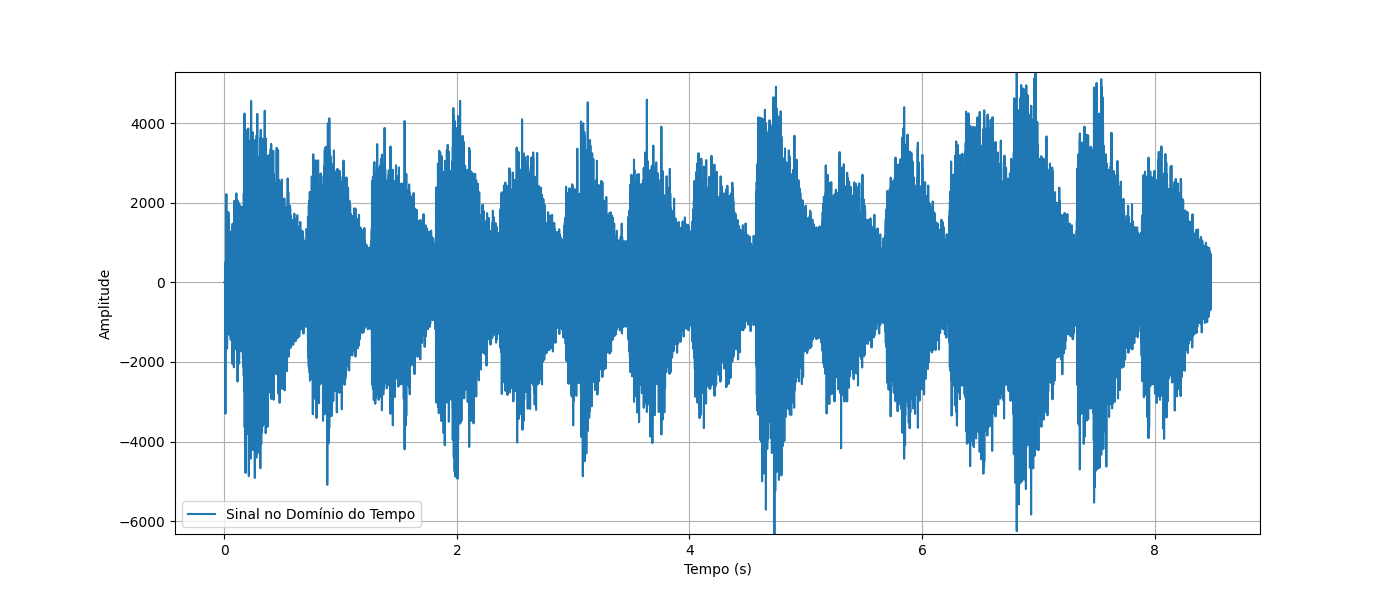
\includegraphics[width=0.7\textwidth]{figuras/fig71.png}
%     \caption{\textit{reverb} com 25 dB após 1 segundo}
%     \label{fig71}
% \end{figure}

% Em seguida, o botão de parâmetro de efeito foi ajustado para que 25 dB permanecessem após 1 segundo da amostra atual da música. Na Figura \ref{fig71}, observa-se a repetição de trechos da música devido à aplicação do efeito.


% %\newpage
% \begin{figure}[h]
%     \centering
%     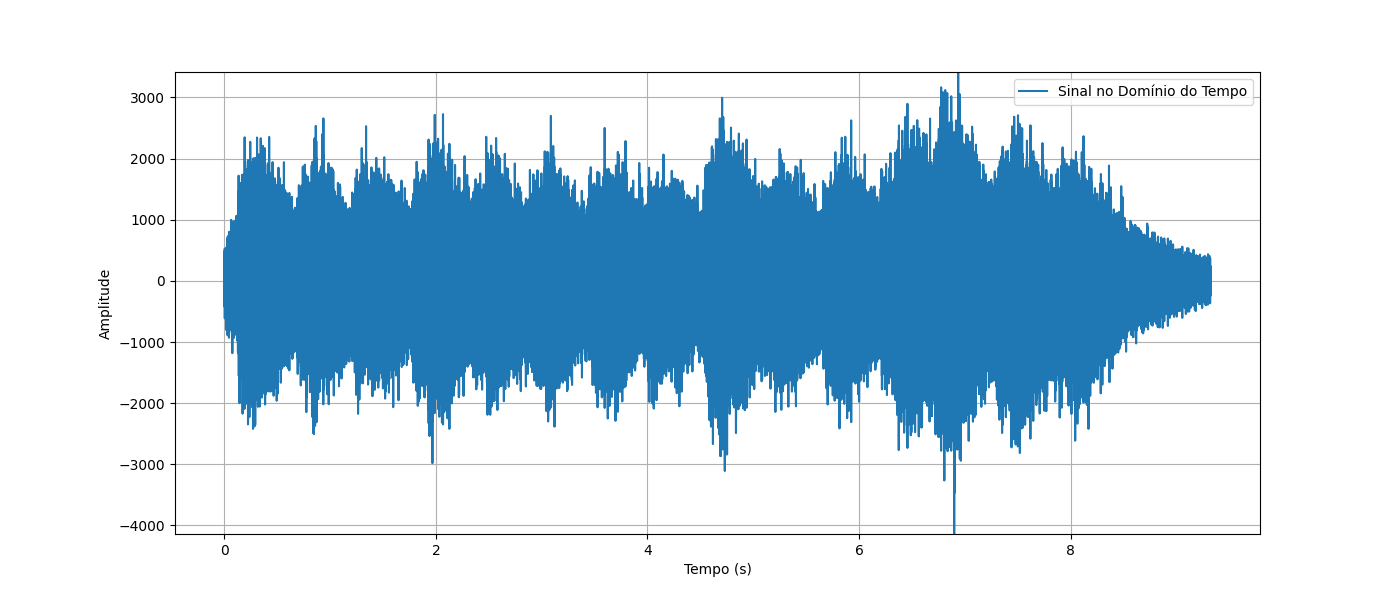
\includegraphics[width=0.7\textwidth]{figuras/fig72.png}
%     \caption{\textit{reverb} com 50 dB após 1 segundo}
%     \label{fig72}
% \end{figure}

% Com o aumento do ganho, o efeito de \textit{reverb} torna-se mais perceptível. Na Figura \ref{fig72}, é possível observar uma maior presença do efeito, com um aumento na amplitude do sinal ao longo do tempo.

% \begin{figure}[h]
%     \centering
%     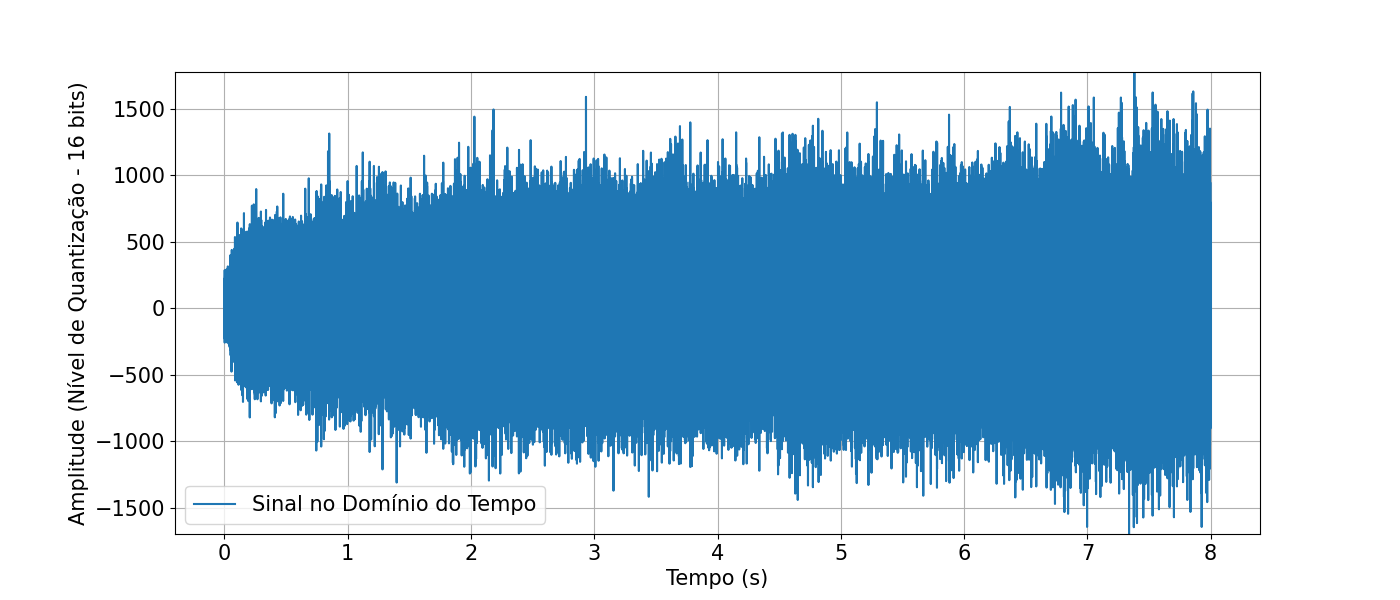
\includegraphics[width=0.7\textwidth]{figuras/fig73.png}
%     \caption{\textit{reverb} com 100 dB após 1 segundo}
%     \label{fig73}
% \end{figure}

% Finalmente, ao configurar 100 dB de ganho após 1 segundo, como mostrado na Figura \ref{fig73}, o efeito de \textit{reverb} é ainda mais pronunciado, resultando em um som com pouca definição. Isso indica que uma grande quantidade de som permaneceu, comprometendo a clareza da música.

\subsubsection*{\textit{Delay}}

O efeito de \textit{delay} consiste em repetir o sinal após um determinado intervalo de tempo. A Fig. \ref{fig74} ilustra o comportamento do efeito com diferentes configurações de atraso.

%\newpage
\begin{figure}[htpb]
    \centering
    % Subfigura a - Delay 0 ms
    \begin{minipage}[b]{0.7\textwidth}
        \centering
        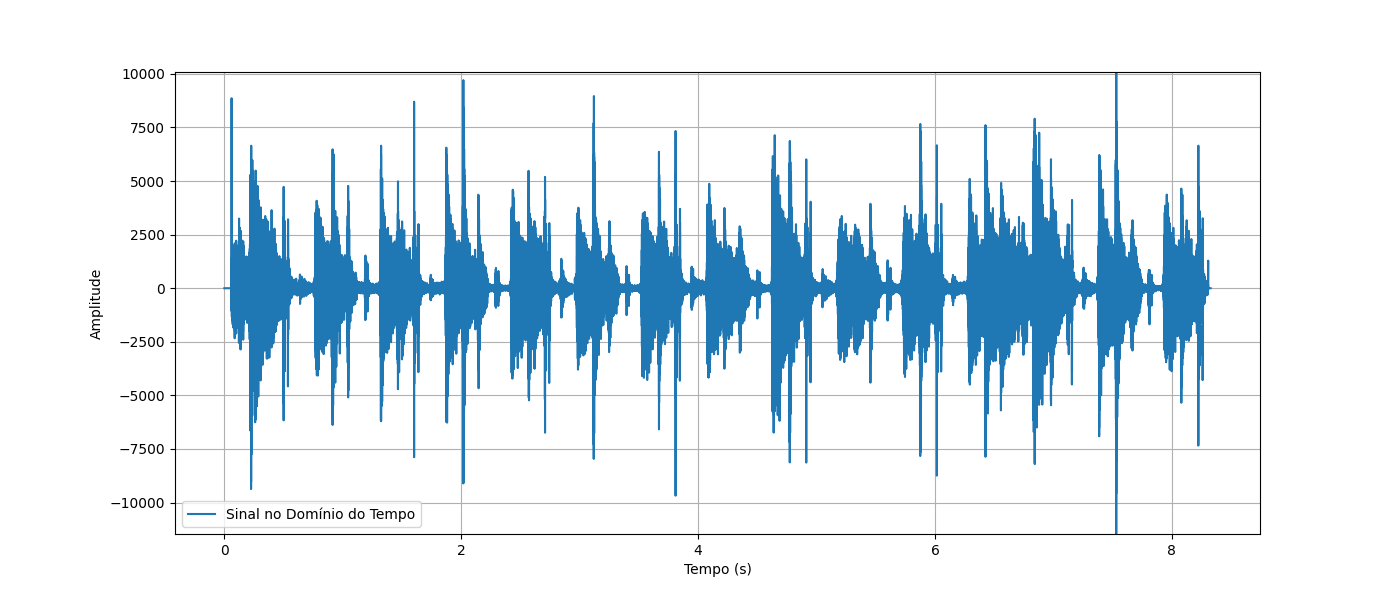
\includegraphics[width=\textwidth]{figuras/fig74.png}
        \vspace{0.3cm} % Espaço entre imagem e sublegenda
        (a) Delay 0 ms.
    \end{minipage}
    \hspace{0.5cm} % Espaço horizontal entre as figuras

    % Subfigura b - Delay 250 ms
    \begin{minipage}[b]{0.7\textwidth}
        \centering
        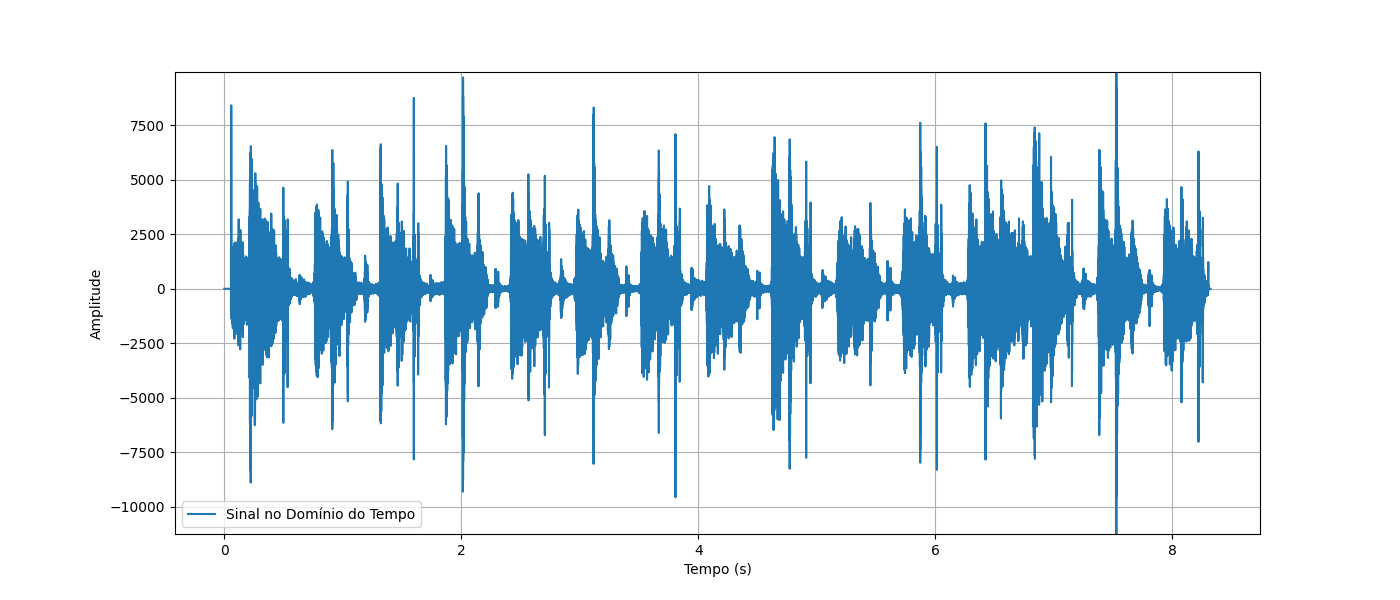
\includegraphics[width=\textwidth]{figuras/fig75.png}
        \vspace{0.3cm} % Espaço entre imagem e sublegenda
        (b) Delay 250 ms.
    \end{minipage}
    
    \vspace{0.5cm} % Espaço vertical entre as linhas de figuras

    % Subfigura c - Delay 500 ms
    \begin{minipage}[b]{0.7\textwidth}
        \centering
        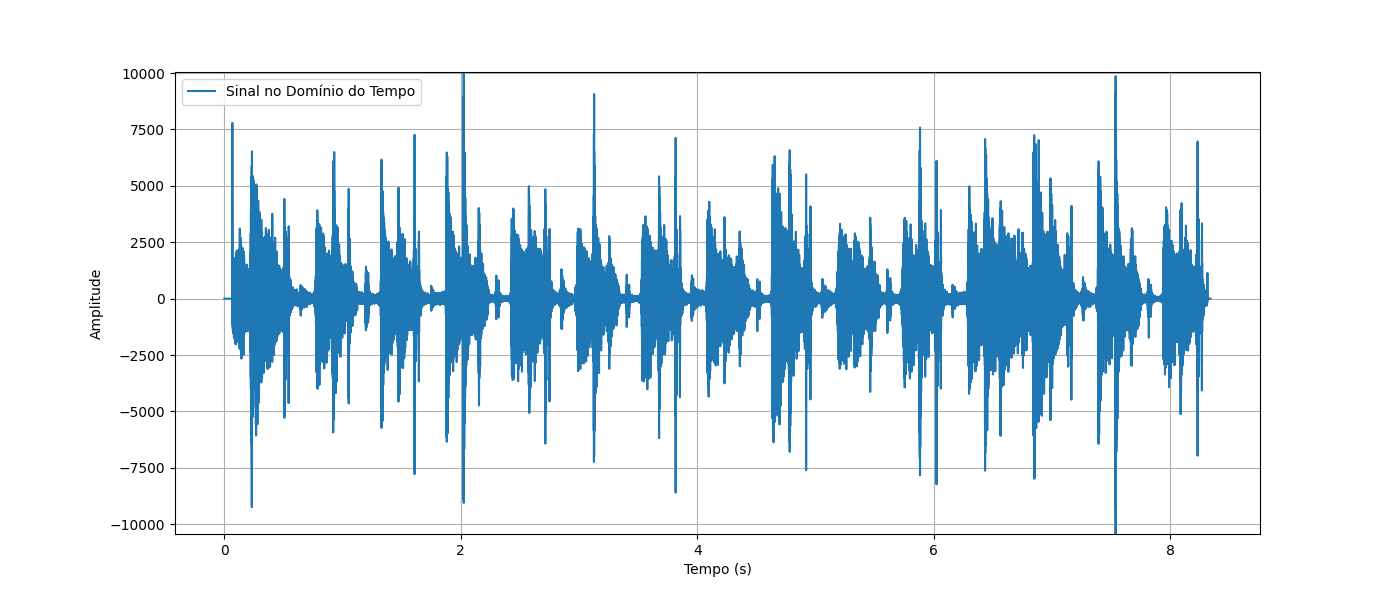
\includegraphics[width=\textwidth]{figuras/fig76.png}
        \vspace{0.3cm} % Espaço entre imagem e sublegenda
        (c) Delay 500 ms.
    \end{minipage}
    \hspace{0.5cm} % Espaço horizontal entre as figuras

    % Subfigura d - Delay 1000 ms
    \begin{minipage}[b]{0.7\textwidth}
        \centering
        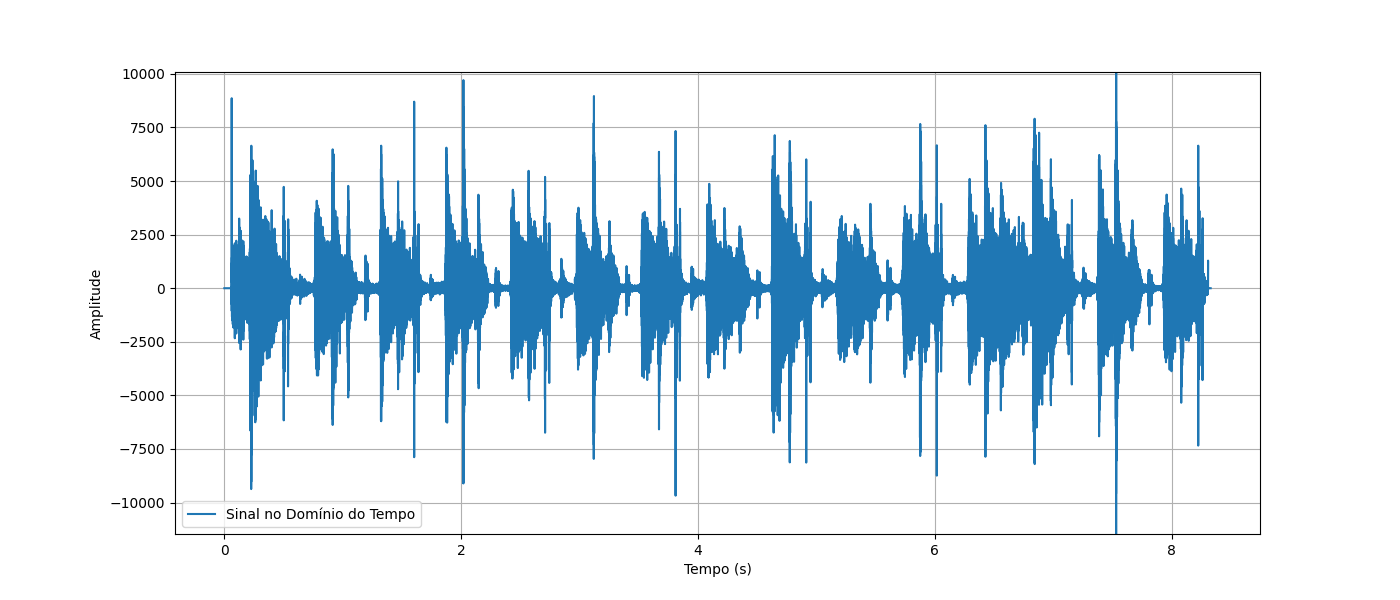
\includegraphics[width=\textwidth]{figuras/fig77.png}
        \vspace{0.3cm} % Espaço entre imagem e sublegenda
        (d) Delay 1000 ms.
    \end{minipage}

    % Legenda geral
    \caption{Sinal com efeitos de \textit{delay} de 0, 250, 500 e 1000 ms.}
    \label{fig74}
\end{figure}

% Na Figura \ref{fig74}, foi configurado um \textit{delay} de 0 ms. Nesse caso, a cópia do sinal é obtida imediatamente, sem atraso.

% \begin{figure}[h]
%   \centering
%     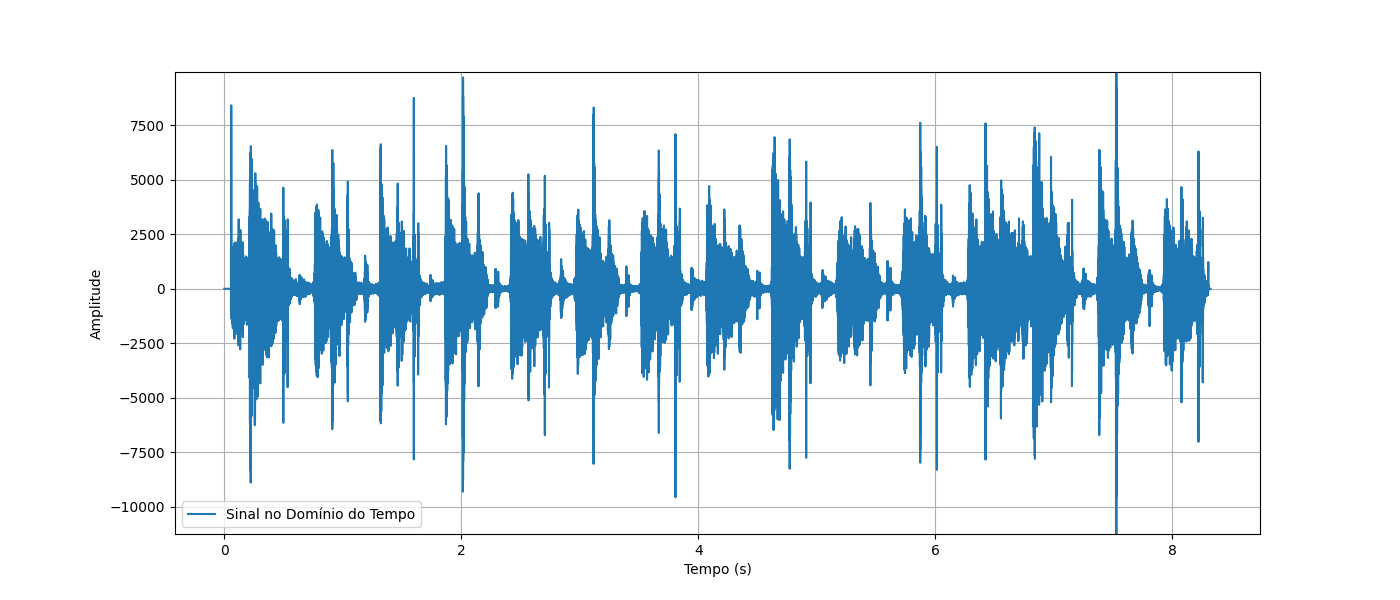
\includegraphics[width=0.7\textwidth]{figuras/fig75.png}
%   \caption{\textit{delay} de 250 ms}
%   \label{fig75}
% \end{figure}

% Na Figura \ref{fig75}, um \textit{delay} de 250 ms foi configurado. Aqui, a cópia do sinal é reproduzida com um atraso de 250 ms em relação ao sinal original.

% \begin{figure}[h]
%   \centering
%     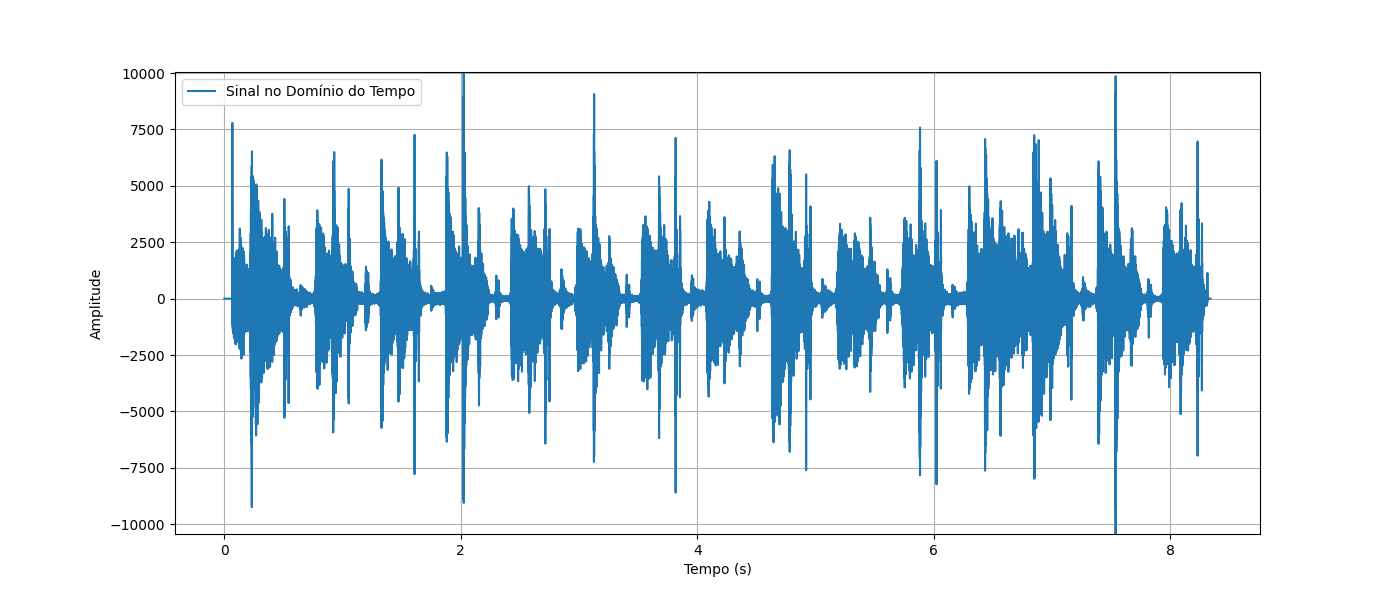
\includegraphics[width=0.7\textwidth]{figuras/fig76.png}
%   \caption{\textit{delay} de 500 ms}
%   \label{fig76}
% \end{figure}

% Na Figura \ref{fig76}, o \textit{delay} foi configurado para 500 ms. Neste caso, a cópia do sinal é reproduzida com um atraso de 500 ms em relação ao sinal original.

%\newpage
% \begin{figure}[h]
%   \centering
%     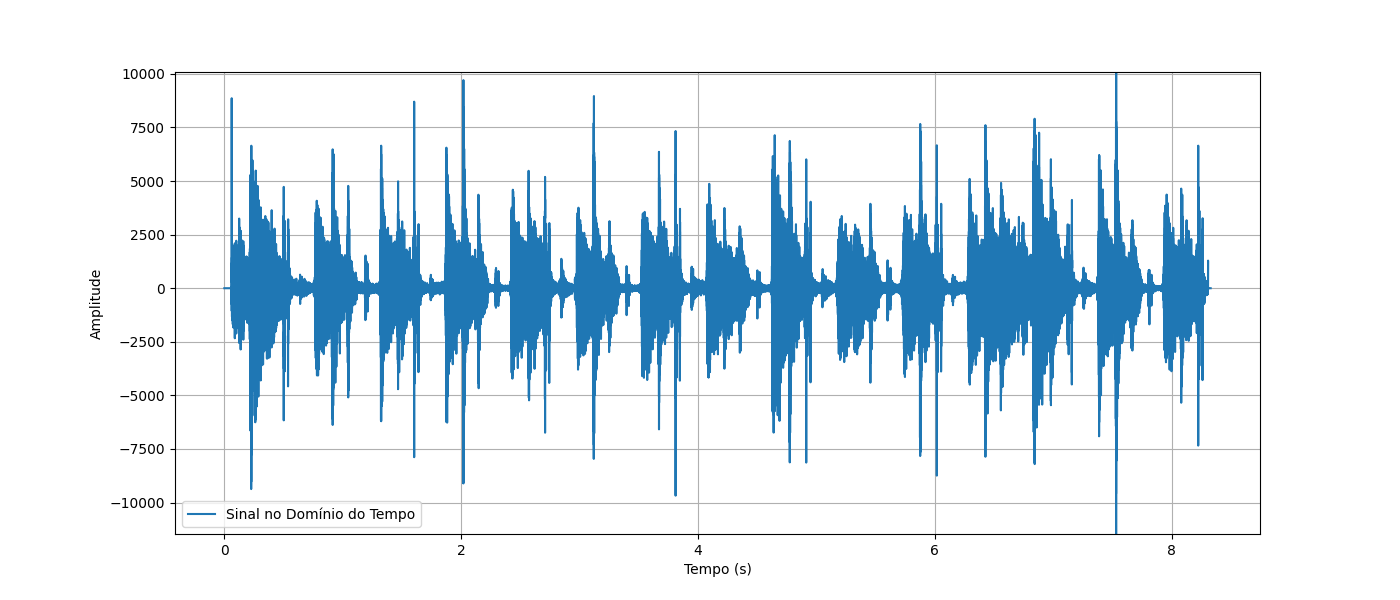
\includegraphics[width=0.7\textwidth]{figuras/fig77.png}
%   \caption{\textit{delay} de 1000 ms}
%   \label{fig77}
% \end{figure}

% Na Figura \ref{fig77}, foi configurado um \textit{delay} de 1000 ms. A cópia do sinal é reproduzida com um atraso de 1000 ms em relação ao sinal original.


\section{Sistema definitivo}

Nessa seção dos resultados, serão apresentadas as metodologias utilizadas para se obter os sinais de áudio para validar a funcionalidade da filtragem e dos efeitos. A estrutura será similar àquela feita para os sinais obtidos do \textit{PureData} para que um paralelo seja estabelecido a fim de compreender melhor os resultados obtidos. Resultados em formato de vídeo para a visualização do pleno funcinamento do sistema estão disponíveis no \textit{README} no \textit{GitHub} do projeto, disponível no \textit{link}: \href{https://github.com/joselitopradomarques/tcc}{Repositório do TCC}.


\subsection{Filtragem}


% Conjunto 1 - Filtro de 20 Hz
\begin{figure}[htpb]
    \centering
    % Subfigura a - Domínio do Tempo
    \begin{minipage}[b]{0.7\textwidth}
        \centering
        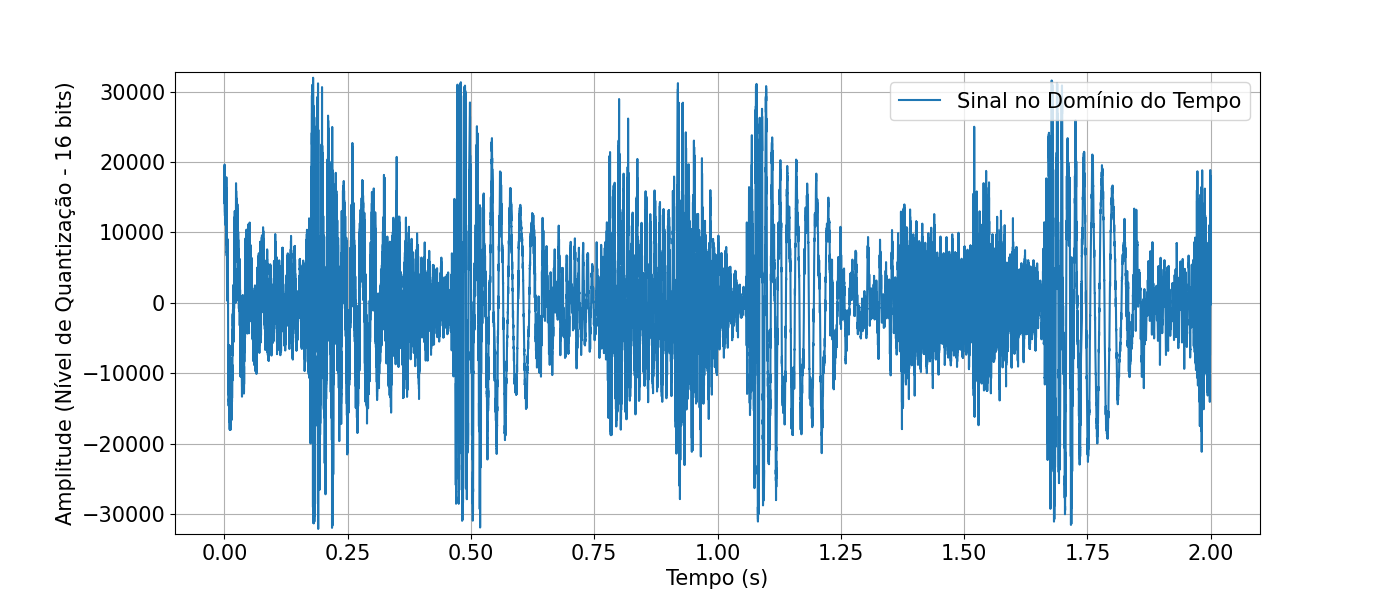
\includegraphics[width=\textwidth]{figuras/fig81.png}
        \vspace{0.3cm} % Espaço entre imagem e sublegenda
        (a) Música 1 no domínio do tempo com filtro de 20 Hz.
    \end{minipage}
    \hspace{0.5cm} % Espaço horizontal entre as figuras

    % Subfigura b - Domínio da Frequência
    \begin{minipage}[b]{0.75\textwidth}
        \centering
        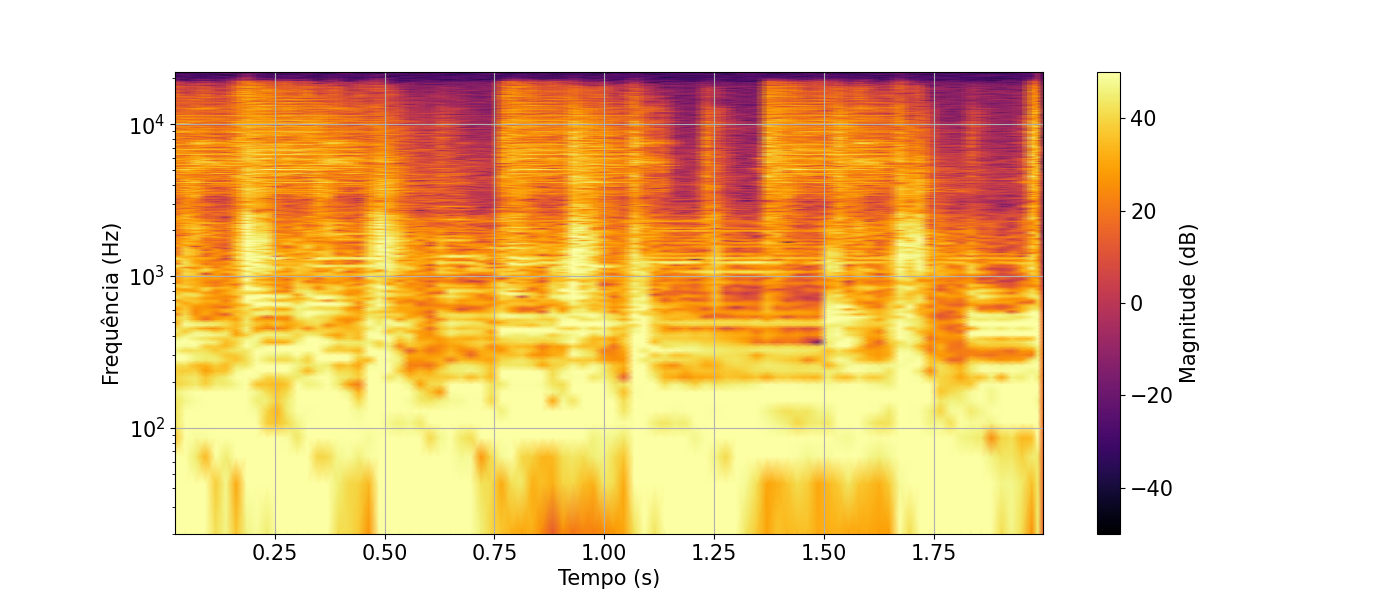
\includegraphics[width=\textwidth]{figuras/fig82.png}
        \vspace{0.3cm} % Espaço entre imagem e sublegenda
        (b) Música 1 no domínio da frequência com filtro de 20 Hz.
    \end{minipage}

    % Legenda geral
    \caption{Música 1 nos domínios do tempo e da frequência, com filtro de 20 Hz.}
    \label{fig81}
\end{figure}

% Conjunto 2 - Filtro de 303 Hz
\begin{figure}[htpb]
    \centering
    % Subfigura a - Domínio do Tempo
    \begin{minipage}[b]{0.7\textwidth}
        \centering
        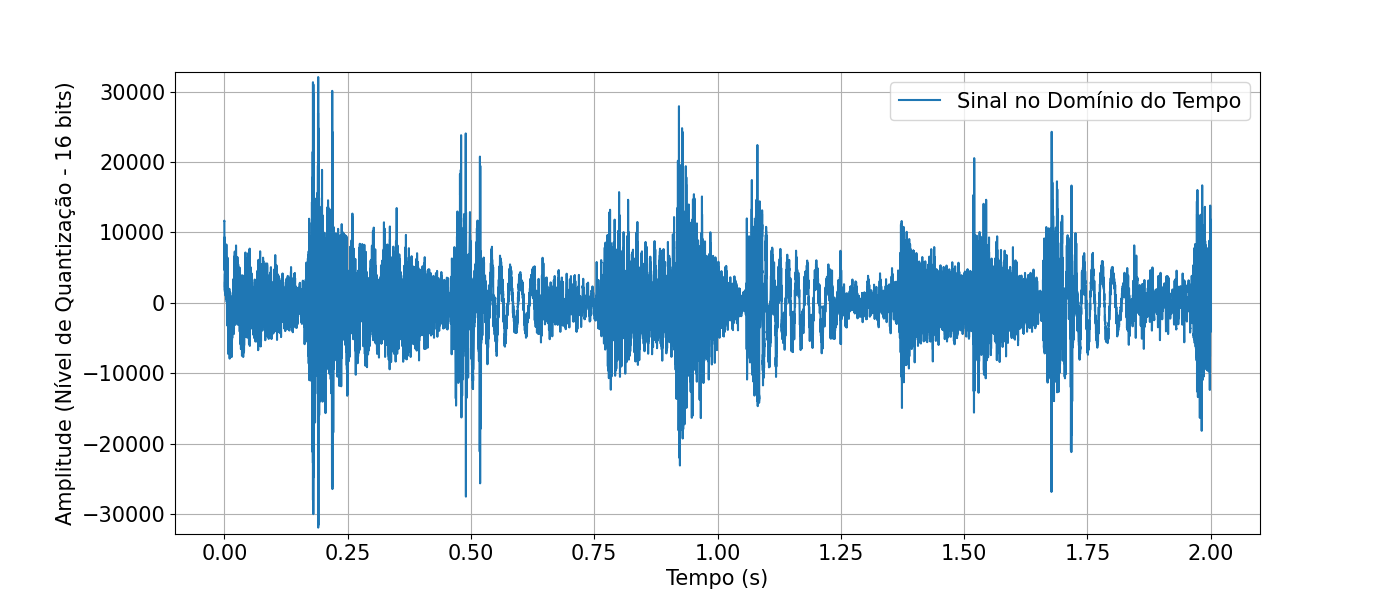
\includegraphics[width=\textwidth]{figuras/fig83.png}
        \vspace{0.3cm} % Espaço entre imagem e sublegenda
        (a) Música 1 no domínio do tempo com frequência de corte de 303 Hz.
    \end{minipage}
    \hspace{0.5cm} % Espaço horizontal entre as figuras

    % Subfigura b - Domínio da Frequência
    \begin{minipage}[b]{0.75\textwidth}
        \centering
        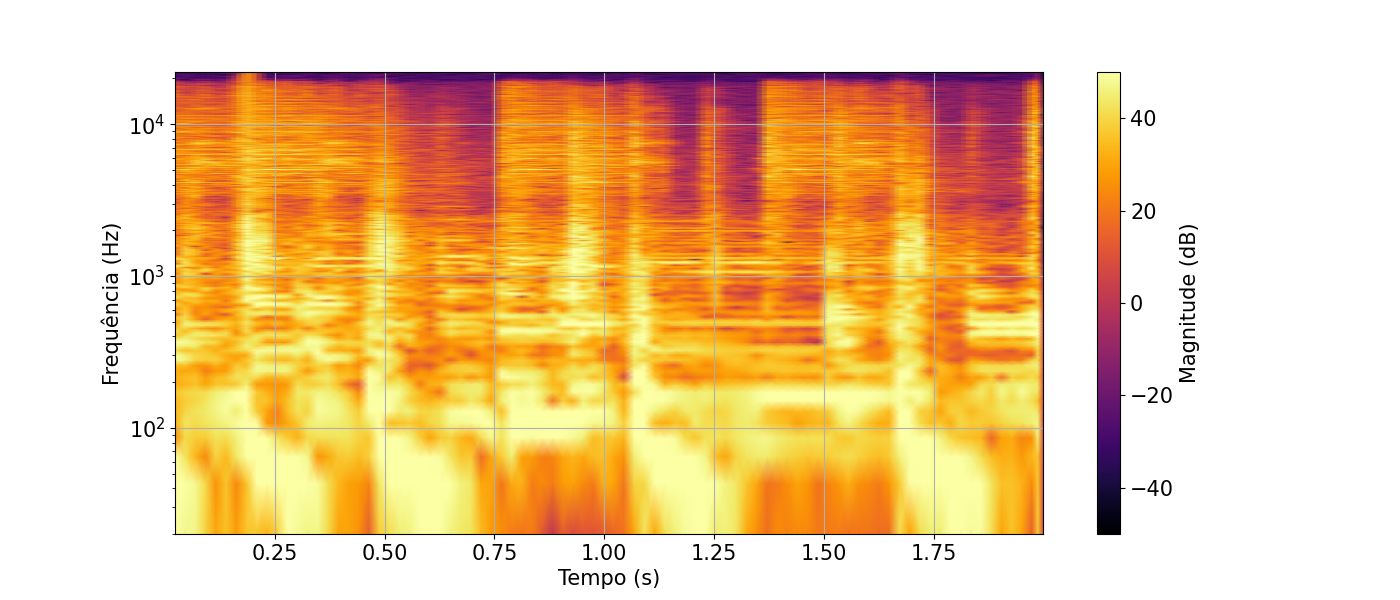
\includegraphics[width=\textwidth]{figuras/fig84.png}
        \vspace{0.3cm} % Espaço entre imagem e sublegenda
        (b) Música 1 no domínio da frequência com frequência de corte de 303 Hz.
    \end{minipage}

    % Legenda geral
    \caption{Música 1 nos domínios do tempo e da frequência, com frequência de corte de 303 Hz.}
    \label{fig83}
\end{figure}

% Conjunto 3 - Filtro de 4015 Hz
\begin{figure}[htpb]
    \centering
    % Subfigura a - Domínio do Tempo
    \begin{minipage}[b]{0.7\textwidth}
        \centering
        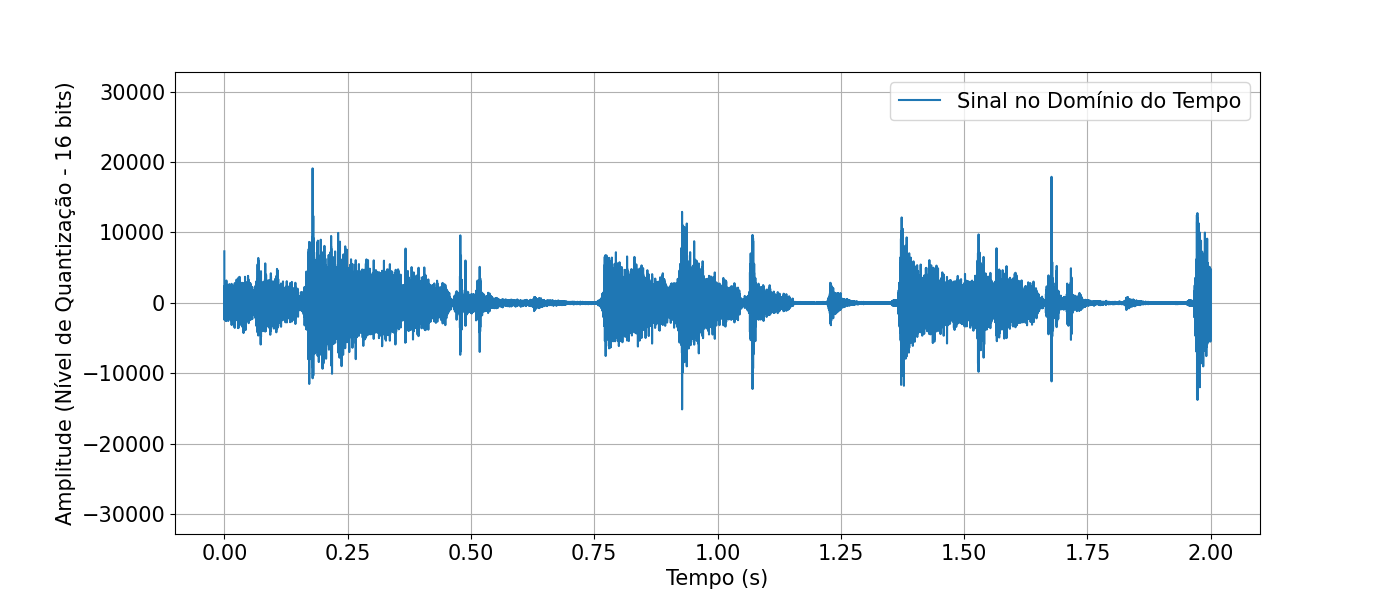
\includegraphics[width=\textwidth]{figuras/fig85.png}
        \vspace{0.3cm} % Espaço entre imagem e sublegenda
        (a) Música 1 no domínio do tempo com frequência de corte de 4015 Hz.
    \end{minipage}
    \hspace{0.5cm} % Espaço horizontal entre as figuras

    % Subfigura b - Domínio da Frequência
    \begin{minipage}[b]{0.7\textwidth}
        \centering
        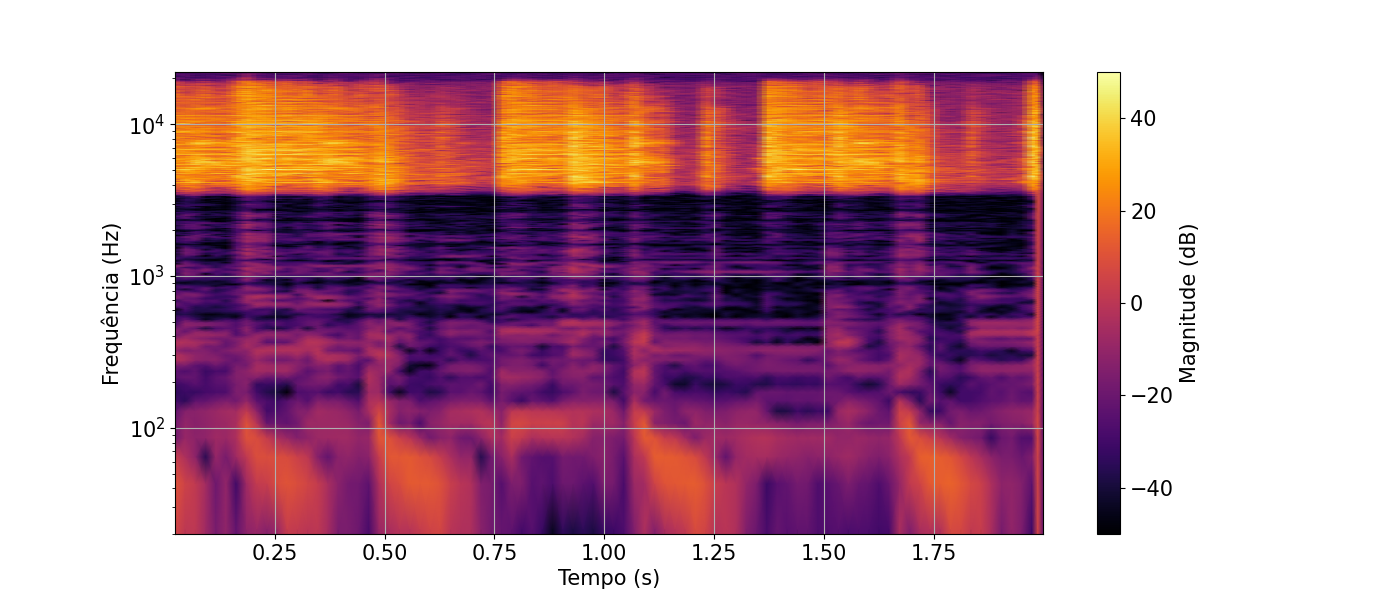
\includegraphics[width=\textwidth]{figuras/fig86.png}
        \vspace{0.3cm} % Espaço entre imagem e sublegenda
        (b) Música 1 no domínio da frequência com frequência de corte de 4015 Hz.
    \end{minipage}

    % Legenda geral
    \caption{Música 1 nos domínios do tempo e da frequência, com frequência de corte de 4015 Hz.}
    \label{fig85}
\end{figure}

% Conjunto 4 - Filtro de 22050 Hz
\begin{figure}[htpb]
    \centering
    % Subfigura a - Domínio do Tempo
    \begin{minipage}[b]{0.7\textwidth}
        \centering
        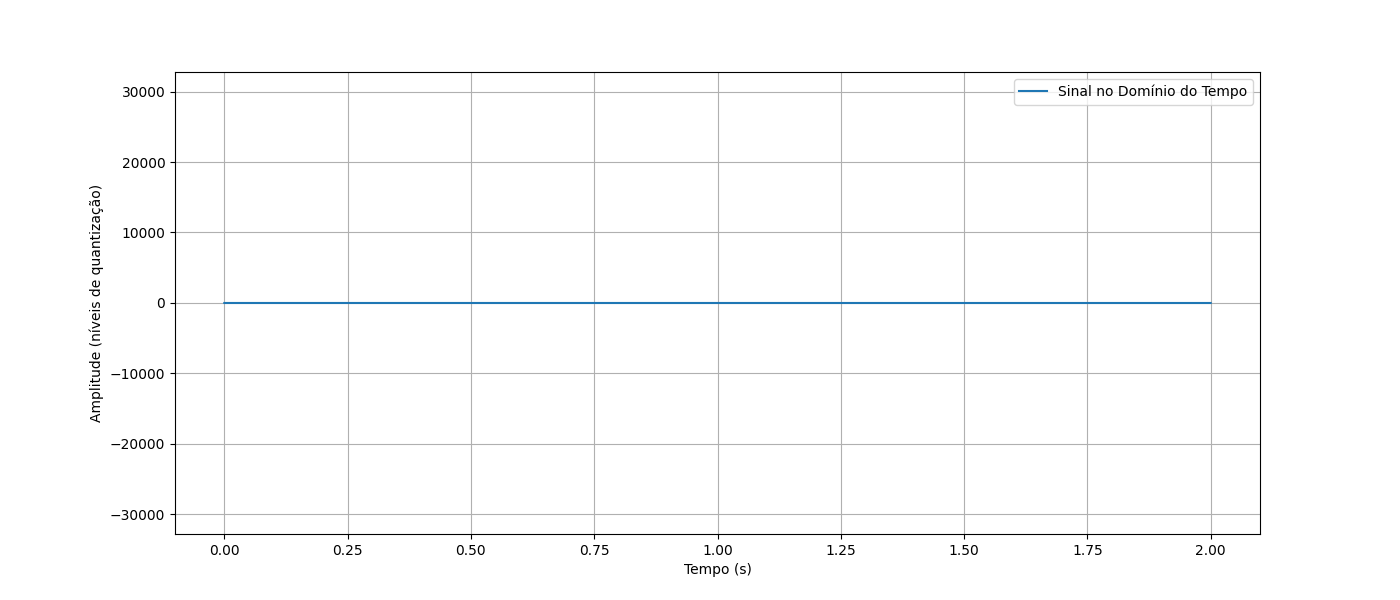
\includegraphics[width=\textwidth]{figuras/fig87.png}
        \vspace{0.3cm} % Espaço entre imagem e sublegenda
        (a) Música 1 no domínio do tempo com frequência de corte de 22050 Hz.
    \end{minipage}
    \hspace{0.5cm} % Espaço horizontal entre as figuras

    % Subfigura b - Domínio da Frequência
    \begin{minipage}[b]{0.7\textwidth}
        \centering
        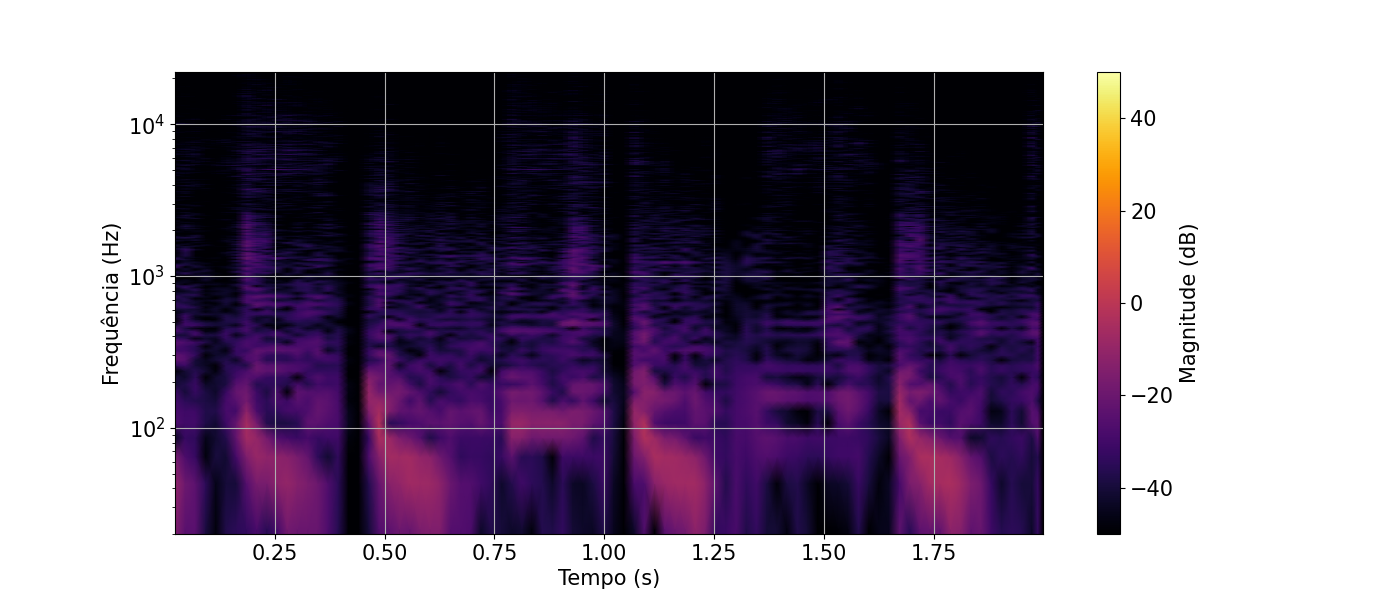
\includegraphics[width=\textwidth]{figuras/fig88.png}
        \vspace{0.3cm} % Espaço entre imagem e sublegenda
        (b) Música 1 no domínio da frequência com frequência de corte de 22050 Hz.
    \end{minipage}

    % Legenda geral
    \caption{Música 1 nos domínios do tempo e da frequência, com frequência de corte de 22050 Hz.}
    \label{fig87}
\end{figure}


Como a conversão analógico digital de 8 \textit{bits} das frequências de corte limita a quantidade de pontos possíveis, para que essa análise se assemelhe àquela feita na prova de conceito, utilizou-se frequências de corte que se aproximassem mais daquelas utilizadas, que foram: 20 Hz, 300 Hz, 4 kHz e 22050 Hz, de forma que as frequências de corte utilizadas nesta análise foram: 20 Hz, 303 Hz, 4015 Hz e 22050 Hz. Nos resultados da prova de conceito, a filtragem foi analisada no ponto 0 Hz, mas como o filtro foi implementado para funcionar na banda de som audível, ou seja, entre 20 e 22050 Hz, a análise neste ponto não foi possível, mas como os sinais são confinados na banda de som audível, o resultado esperado para 0 Hz seria o mesmo daquele obtido para 20 Hz. 

Nos resultados da prova de conceito, um sinal foi obtido após a filtragem de um canal apenas para que a análise em frequência pudesse ser realizada de forma que se pudesse analisar a efetividade da filtragem em um sinal específico. Nesta etapa, como o código filtra os dois áudios e em seguida os unifica, um áudio "branco", composto de amostras nulas, foi gerado para que apenas a influência de um canal seja percebido. 
Além disso, o mesmo sinal de teste utilizado para a prova de conceito foi utilizada nesses testes \cite{track01}.

% Para a obtenção de um arquivo \textit{wav} que possa ser analisado, uma função que acumula os \textit{buffers} processados e ao fim o salva em um arquivo \textit{wav} foi implementada.

% Portanto, a análise a seguir será feita a partir de um sinal de teste, contemplando uma lista de frequências de corte, de forma que uma análise no domínio do tempo dos dois primeiros segundos na faixa de amostras quantizadas de 16 \textit{bits} e outra para verificar a composição dos componentes em frequência utilizando a STFT. 

A análise da filtragem foi feita elencando frequências de corte para verificar a efetividade do processamento de forma que toda a banda pudesse ser contemplada. Assim, iniciou-se com a frequência de corte mais baixa, que é a de 20 Hz (Fig. \ref{fig81}). 

Alterando-se as frequências de corte para 303 Hz (Fig. \ref{fig83}), percebe-se que componentes cujas variações eram mais lentas foram eliminadas, resultado esperado após realizar uma filtragem passa-altas em 303 Hz. Ao escutar esse sinal, percebeu-se que boa parte dos sons mais graves foram bastante atenuados. Outro ponto importante para a análise da efetividade da filtragem é que a amplitude de sinais de frequências maiores foi mantida, que se pode verificar com os picos presentes nessa Figura. Repare que no sinal original há uma faixa bastante definida em torno de 100 Hz (Fig. \ref{fig81}b), e a mesma, após a filtragem, já se encontra bastante atenuada.

Na frequência de corte em 4015 HZ (Fig. \ref{fig85}), pode-se ver que as componentes entre 20 e 4015 Hz foram atenuadas, restando ao sinal apenas as componentes dessa banda superior. Com isso, o sinal fica com variações de altas frequências cujas amplitudes são menores. Ao realizar a escuta do sinal resultante, a saída pode ser descrita como se um sinal estivesse apenas ecoado, com sinais estridentes, característicos de altas frequências. 
Na frequência de corte de 22050 Hz (Fig. \ref{fig87}), pode-se ver que todas as componentes do sinal são atenuadas. 

Portanto, com essas análises dos sinais tanto no tempo quanto na frequência para variados pontos, atesta-se a eficiência do filtro utilizado bem como a sua configuração feita com o janelamento e a ordem dos filtros.

%, domínio do tempo, e \ref{fig82}, para o domínio da frequência.
%Na Figura \ref{fig81}, encontra-se o sinal original, obtido da música \cite{track01}, janelado a um intervalo de dois segundos, e representado por valores quantizados de 16 \textit{bits}. %Por ser o dado original, essa representação será uma referência para a aplicação das filtragens a serem realizadas em frequências de corte superiores.
% Na Figura \ref{fig82}, encontra-se o sinal original no domínio da frequência, mas com os mesmos parâmetros da Figura anterior. Essa representação através de um mapa de calor também serve como referência para as mudanças que serão realizadas em filtragens com frequência de corte superiores. 




% \begin{figure}[h]
%     \centering
%     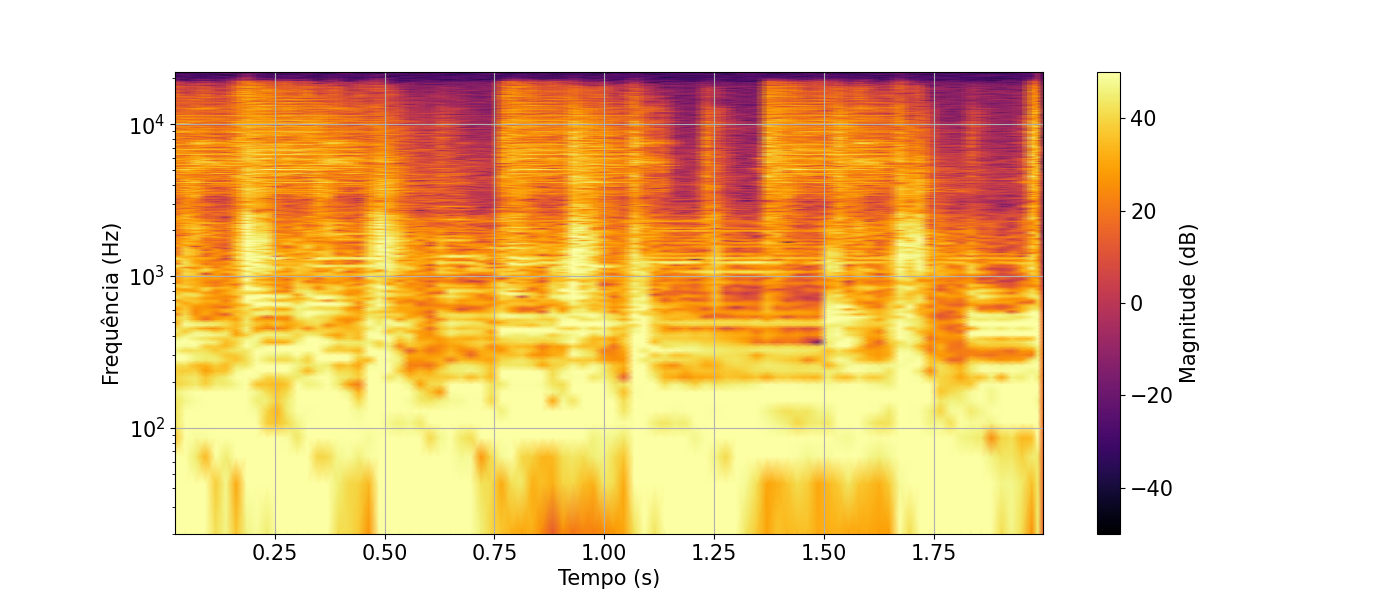
\includegraphics[width=0.7\textwidth]{figuras/fig82.png}
%     \caption{Música 1 no domínio da frequência sem filtragem}
%     \label{fig82}
% \end{figure}

% Em seguida, alterou-se a frequência de corte para 303 Hz, pois foi o valor mais próximo dos 300 Hz utilizado na prova de conceito. Assim, na Figura \ref{fig83}, percebe-se que componentes cujas variações eram mais lentas foram eliminadas, resultado esperado após realizar uma filtragem passa-altas em 303 Hz. Ao escutar esse sinal, percebeu-se que boa parte dos sons mais graves foram bastante atenuados. Outro ponto importante para a análise da efetividade da filtragem é que a amplitude de sinais de frequências maiores foi mantida, que se pode verificar com os picos presentes nessa Figura.


% Para validar a filtragem realizada nas componentes de baixa frequência, utilizou-se também o STFT em forma de mapa de calor. Ao se comparar as Figuras \ref{fig82} (sinal original) e \ref{fig84} (sinal filtrado a 303 Hz), valida-se a filtragem realizada nessa banda visto que no sinal original há uma faixa bastante definida em torno de 100 Hz, e a mesma, após a filtragem, já se encontra bastante atenuada. Em contrapartida, percebe-se também que as componentes de alta frequência continuam intactas. 

% % \begin{figure}[h]
% %     \centering
% %     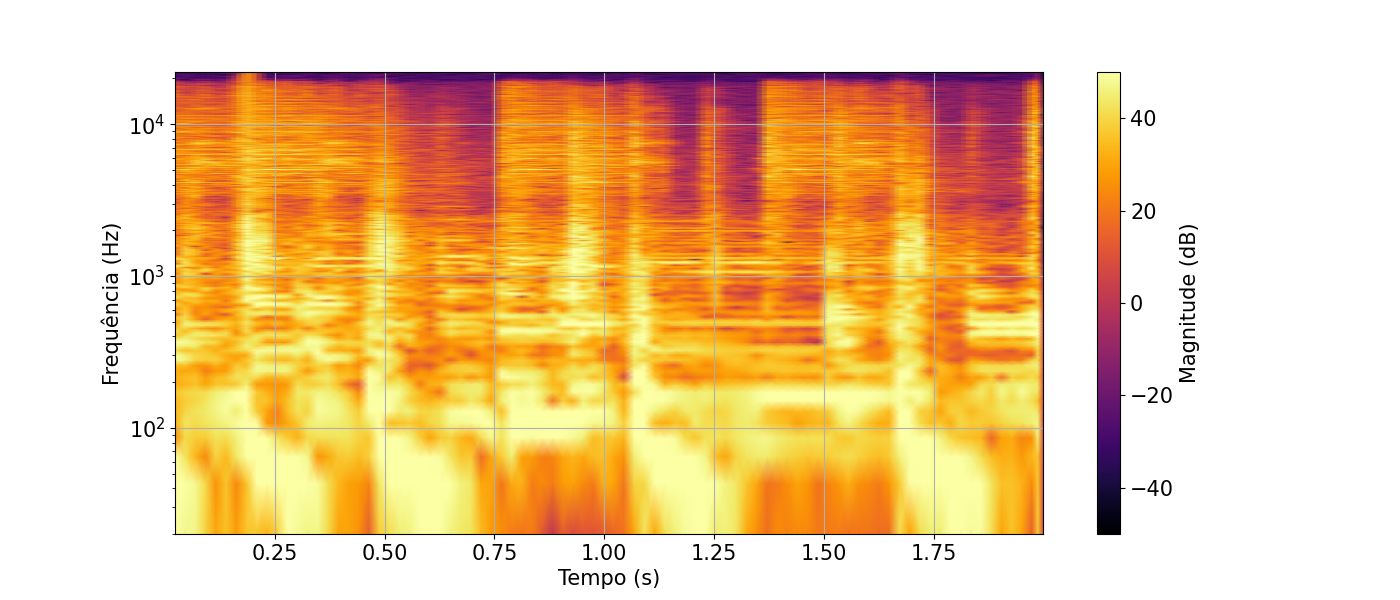
\includegraphics[width=0.7\textwidth]{figuras/fig84.png}
% %     \caption{Música 1 no domínio da frequência com frequência de corte 303 Hz}
% %     \label{fig84}
% % \end{figure}

% Para continuar a validação da filtragem, a frequência de corte foi alterada para 4015 Hz. À essa frequência, espera-se que boa parte da energia contida em um sinal de música tenha sido eliminada. Ao analisar a Figura \ref{fig85}, esse fenômeno é confirmado visto que as componentes entre 20 e 4015 foram atenuadas, restando ao sinal apenas as componentes dessa banda superior. Com isso, o sinal fica com variações de altas frequências cujas amplitudes são menores. Ao realizar a escuta do sinal resultante, a saída pode ser descrita como se um sinal estivesse apenas ecoado, com sinais estridentes, característicos de altas frequências. 



% Resquícios de componentes de alta frequência e a atenuação da banda inferior são vistos com mais facilidade na STFT da Figura \ref{fig86}, na qual os sinais abaixos de 4000 Hz tem sua magnitude reduzidas à faixa de -20 a -40 dB.


% % \begin{figure}[h]
% %     \centering
% %     \includegraphics[width=0.7\textwidth]{figuras/fig86.png}
% %     \caption{Música 1 no domínio da frequência com frequência de corte 4015 Hz}
% %     \label{fig86}
% % \end{figure}

% Por fim, para se atestar a eficiência da eliminação completa de um canal, utiliza-se a frequência de corte de 22050 Hz, pois, sendo um passa-altas aplicado a um final limitado a essa mesma frequência, todas as componentes do sinal são atenuadas. Na Figura \ref{fig87}, essa anulação do canal pode ser atestada visto que o sinal resultante aparece nulo. 


% A representação no domínio da frequência dessa filtragem atesta que todas componentes foram atenuadas para a faixa de -40 dB de magnitude. Além disso, ao escutar o sinal de saída, não se percebe a presença de sinal algum. 

% % \begin{figure}[h]
% %     \centering
% %     \includegraphics[width=0.7\textwidth]{figuras/fig88.png}
% %     \caption{Música 1 no domínio da frequência com frequência de corte 22050 Hz}
% %     \label{fig88}
% % \end{figure}

% Portanto, com essas análises dos sinais tanto no tempo quanto na frequência para variados pontos, atesta-se a eficiência do filtro utilizado bem como a sua configuração feita com o janelamento e a ordem dos filtros.

\subsection{Efeitos}

Na implementação do sistema, a lógica de presença dos efeitos foi alterada para dar mais liberdade à mixagem. Antes, o efeito era controlado pela frequência de corte, que determinava o volume do efeito a ser adicionado no sinal de saída. Porém, nesta implementação, o usuário pode escolher a intensidade através de um potenciômetro.

Quando se diz intensidade, a variável chamada \textit{wetness} é invocada, de forma que esse parâmetro indica quanto sinal seco (sinal original) e "molhado" (sinal com efeito) estarão presentes no sinal final. Quando maior o \textit{wetness}, mais o efeito estará presente. 

Os resultados em relação aos efeitos na prova de conceito foram obtidos variando o volume do efeito, que consequentemente determina a presença do efeito no sinal final. Neste caso, o volume deu lugar ao \textit{wetness}, de forma que os resultados para os efeitos foram obtidos para os seguintes valores de \textit{wetness}: 0.0, 0.33, 0.66 e 1.00. 

\subsubsection*{\textit{Delay}}


\begin{figure}[htpb]
    \centering
    % Subfigura a - Wetness 0.0
    \begin{minipage}[b]{0.7\textwidth}
        \centering
        \includegraphics[width=\textwidth]{figuras/fig89.png}
        \vspace{0.3cm} % Espaço entre imagem e sublegenda
        (a) Música 1 com \textit{delay} e wetness 0.0.
    \end{minipage}
    \hspace{0.5cm} % Espaço horizontal entre as figuras

    % Subfigura b - Wetness 0.33
    \begin{minipage}[b]{0.7\textwidth}
        \centering
        \includegraphics[width=\textwidth]{figuras/fig90.png}
        \vspace{0.3cm} % Espaço entre imagem e sublegenda
        (b) Música 1 com \textit{delay} e wetness 0.33.
    \end{minipage}
    
    \vspace{0.5cm} % Espaço vertical entre as linhas de figuras

    % Subfigura c - Wetness 0.66
    \begin{minipage}[b]{0.7\textwidth}
        \centering
        \includegraphics[width=\textwidth]{figuras/fig91.png}
        \vspace{0.3cm} % Espaço entre imagem e sublegenda
        (c) Música 1 com \textit{delay} e wetness 0.66.
    \end{minipage}
    \hspace{0.5cm} % Espaço horizontal entre as figuras

    % Subfigura d - Wetness 1.0
    \begin{minipage}[b]{0.7\textwidth}
        \centering
        \includegraphics[width=\textwidth]{figuras/fig92.png}
        \vspace{0.3cm} % Espaço entre imagem e sublegenda
        (d) Música 1 com \textit{delay} e wetness 1.0.
    \end{minipage}

    % Legenda geral
    \caption{Música 1 com \textit{delay} a valores de \textit{wetness} de 0,0, 0,33, 0,66 e 1,0.}
    \label{fig89}
\end{figure}



Para atestar a efetividade da implementação do código para o \textit{delay}, obteve-se os sinais de saída para cada valor do parâmetro \textit{wetness}. Como esse efeito é baseado na repetição de amostras anteriores, ou o atraso de reprodução de cópias correntes, a representação no domínio do tempo se mostra suficiente para se verificar a atuação do efeito em função do parâmetro de mistura entre o sinal original e o processado pelo efeito. 
Para a realização desses testes, a frequência de corte utilizada na etapa de filtragem foi a de 20 Hz, mantendo praticamente o mesmo sinal que adentrava o filtro. % E da mesma forma como foi feito na seção de resultados da filtragem, nessa seção, a primeira Figura também será utilizada como referência para as análises seguintes.

Ao se configurar o parâmetro de mistura como 0,00, entende-se que apenas o sinal original será transmitido pela saída do efeito. Portanto, o sinal presente na Fig. \ref{fig89}a nada mais é que o sinal original, também presente na Figura \ref{fig81}a, porém, com a amplitude dividida pela metade, visto que, ao se unificar os canais 1 e 2, realiza-se uma média entre as amostras. Como o canal 2 possui uma música com componentes nulas, a representação final é basicamente o sinal 1 pela metade. Outro ponto importante é que caso o usuário não queira a presença de efeitos, o parâmetro nulo de \textit{wetness} funciona como uma chave liga-desliga para o efeito utilizado. 


Quando o parâmetro de mistura aumenta, uma combinação linear entre o sinal original e o sinal com efeito é realizada, de forma que se o o \textit{wetness} é 0,33, as amostras do sinal original são multiplicadas por um fator de 0,67, enquanto os sinais dos efeitos são aplicados a um fator de 0,33. Dessa forma, diferente dos resultados de efeito \textit{delay} obtidos pelo \textit{PureData}, nos quais era possível verificar o aumento do atraso conforme o aumento do parâmetro, nesta implementação desse efeito, o aumento do parâmetro de controle não aumenta o atraso, mas sim a presença do sinal processado com o efeito pré-configurado, e diminui os sinais originais. 

Assim, no gráfico da Fig. \ref{fig89}b, a atenuação da amplitude do sinal original é observada, visto que o contorno principal do sinal cai para uma mesma faixa. Junto com o sinal original, encontra-se o sinal atrasado em 0,5 segundo, com uma amplitude de 0,34 do seu valor original. Dessa forma, tanto o sinal original quanto o atrasado se fazem presentes. Ao se escutar o sinal de saída, percebe-se que o efeito de \textit{delay} foi realizado com sucesso, visto que uma sensação de eco é criada. 

% \begin{figure}[h]
%     \centering
%     \includegraphics[width=0.7\textwidth]{figuras/fig90.png}
%     \caption{Música 1 com \textit{delay} a um \textit{wetness} = 0.33 }
%     \label{fig90}
% \end{figure}

Ao aumentar o valor do \textit{wetness} para 0,66, o sinal original decai mais ainda para 0.33 da sua amplitude original, enquanto o sinal com efeitos tem um fator de 0.67, e, com isso, o que se vê no gráfico da Fig. \ref{fig89}c é a maior presença de um sinal atrasado e a queda do sinal original. No sinal de saída, percebe-se mais ainda a sensação de eco provocada por esse efeito.

% \begin{figure}[h]
%     \centering
%     \includegraphics[width=0.7\textwidth]{figuras/fig91.png}
%     \caption{Música 1 com \textit{delay} a um \textit{wetness} = 0.66 }
%     \label{fig91}
% \end{figure}

Ao se definir o valor do \textit{wetness} para 1,00, apaga-se o sinal original, dando espaço apenas ao sinal atrasado. Porém, na implementação desse efeito, existe um fator de \textit{feedback}, que faz com que amostras anteriores sejam realimentadas. Por isso, o sinal final não é apenas um sinal atrasado, fato comprovado na escuta dessas amostras. Então, por mais que o gráfico da Figura \ref{fig89}d dê a entender que o sinal está simplesmente atrasado, ainda há a presença de uma sensação de \textit{delay} devido ao \textit{feedback} criado. Outro ponto importante que pode ser observado é o atraso de 0,5 segundo existente na amostra com efeitos, visto que percebe-se que o sinal se inicia com esse atraso pré-estabelecido.

% \begin{figure}[h]
%     \centering
%     \includegraphics[width=0.7\textwidth]{figuras/fig92.png}
%     \caption{Música 1 com \textit{delay} a um \textit{wetness} = 1.00}
%     \label{fig92}
% \end{figure}

Assim, com esses resultados, foi possível validar a implementação do efeito \textit{delay}, e, apesar que há inúmeras formas de se implementar esse efeito, a forma escolhida, que envolve a definição de um tempo de atraso fixo, com um parâmetro que realiza a ponderação entre o sinal original e o sinal com efeito, se mostrou eficiente para gerar o efeito desejado.

\subsubsection*{\textit{Reverb}}

Da mesma forma como nos resultados para o \textit{delay}, os resultados para o efeito \textit{reverb} foram obtidos variando o valor do parâmetro de mistura \textit{wetness} para os mesmos valores de 0,0, 0,33, 0,66 e 1,0.

Percebe-se muita semelhança entre os resultados para \textit{delay} (Fig. \ref{fig89}) e \textit{reverb} (Fig. \ref{fig93}) para os mesmos casos de parâmetro de mistura. Essa semelhança ocorre devido à forma com que o efeito \textit{reverb} é construído. Enquanto \textit{delay} é um atraso gerado nas amostras correntes, o \textit{reverb} partilha do mesmo princípio mas em mais camadas, visto que esse efeito funciona como se fosse um banco de \textit{delays}. Daí se entende a semelhança entre os dois. Além disso, percebe-se que conforme se aumenta o \textit{wetness}, o sinal do \textit{reverb} se torna menos definido, devido à maior presença do efeito, fazendo com que esse banco de \textit{delays} atua com mais presença.

A primeira representação dos sinais processados dessa seção, Fig. \ref{fig93}a, novamente, é uma represenação do sinal original, de forma que esse traçado é tido como referência para os demais gráficos da Fig. % para os próximos gráficos nos quais são exibidos os comportamentos dos sinais em função do processamento de \textit{reverb} feito.
Devido à construção desse efeito que, em comparação com o \textit{delay}, possui um \textit{feedback} mais suave e distribuído, o sinal resultante não demonstra com clareza a execução do efeito. Porém, pode-se observar a atuação do parâmetro \textit{wetness}, que faz com que a amplitude do sinal original seja atenuada. Nesse caso, como os \textit{delays} são mais numerosos mas mais suaves, a presença do efeito se dá de forma efetiva na escuta do sinal resultante, o que foi comprovado em sua escuta.
% Seguindo a mesma lógica da Figura \ref{fig94}, é possível observar na Figura \ref{fig95} a repetição de grandes blocos de amostras. O som se torna menos definido, fato comprovado na escuta do arquivo final. Além disso, na escuta pôde se observar a intensificação do efeito de reverberação.

\begin{figure}[htpb]
    \centering
    % Subfigura a - Wetness 0.0
    \begin{minipage}[b]{0.7\textwidth}
        \centering
        \includegraphics[width=\textwidth]{figuras/fig93.png}
        \vspace{0.3cm} % Espaço entre imagem e sublegenda
        (a) Música 1 com \textit{reverb} e wetness 0.0.
    \end{minipage}
    \hspace{0.5cm} % Espaço horizontal entre as figuras

    % Subfigura b - Wetness 0.33
    \begin{minipage}[b]{0.7\textwidth}
        \centering
        \includegraphics[width=\textwidth]{figuras/fig94.png}
        \vspace{0.3cm} % Espaço entre imagem e sublegenda
        (b) Música 1 com \textit{reverb} e wetness 0.33.
    \end{minipage}
    
    \vspace{0.5cm} % Espaço vertical entre as linhas de figuras

    % Subfigura c - Wetness 0.66
    \begin{minipage}[b]{0.7\textwidth}
        \centering
        \includegraphics[width=\textwidth]{figuras/fig95.png}
        \vspace{0.3cm} % Espaço entre imagem e sublegenda
        (c) Música 1 com \textit{reverb} e wetness 0.66.
    \end{minipage}
    \hspace{0.5cm} % Espaço horizontal entre as figuras

    % Subfigura d - Wetness 1.0 (erro na repetição de fig95 corrigido)
    \begin{minipage}[b]{0.7\textwidth}
        \centering
        \includegraphics[width=\textwidth]{figuras/fig96.png}
        \vspace{0.3cm} % Espaço entre imagem e sublegenda
        (d) Música 1 com \textit{reverb} e wetness 1.0.
    \end{minipage}

    % Legenda geral
    \caption{Música 1 com \textit{reverb} a valores de \textit{wetness} de 0,0, 0,33, 0,66 e 1,0.}
    \label{fig93}
\end{figure}



% \begin{figure}[h]
%     \centering
%     \includegraphics[width=0.7\textwidth]{figuras/fig94.png}
%     \caption{Música 1 com \textit{reverb} a um \textit{wetness} = 0.33}
%     \label{fig94}
% \end{figure}


% \begin{figure}[h]
%     \centering
%     \includegraphics[width=0.7\textwidth]{figuras/fig95.png}
%     \caption{Música 1 com \textit{reverb} a um \textit{wetness} = 0.66}
%     \label{fig95}
% \end{figure}

Novamente, ao se definir o valor do \textit{wetness} para 1.00, apenas o sinal processado pelo efeito de reverberação é aplicado ao sinal resultante, como se pode ver no gráfico da Fig. \ref{fig93}d. E ao se escutar o arquivo final, percebe-se com clareza o efeito de reverberação, com muitas camadas de ecos aplicadas ao sinal original.

% \begin{figure}[h]
%     \centering
%     \includegraphics[width=0.7\textwidth]{figuras/fig96.png}
%     \caption{Música 1 com \textit{reverb} a um \textit{wetness} = 1.00}
%     \label{fig96}
% \end{figure}

Dessa forma, ao se analisar as representações dos sinais processados no domínio do tempo, observou-se que conforme se aumentou o parâmetro \textit{wetness}, a música perde muita da sua definição, e não se consegue concluir visualmente a presença do efeito de reverberação. Porém, ao se realizar as escutar dos sinais resultantes, conclui-se que o efeito foi aplicado de forma satisfatória.